\def\year{2018}\relax
%File: formatting-instruction.tex
\documentclass[letterpaper]{article} %DO NOT CHANGE THIS
\usepackage{aaai18}  %Required
\usepackage{times}  %Required
\usepackage{helvet}  %Required
\usepackage{courier}  %Required
\usepackage{url}  %Required
\usepackage{graphicx}  %Required
\frenchspacing  %Required

%\usepackage[titletoc,toc,title]{appendix}
\usepackage{amssymb}
\usepackage{amsthm}
\usepackage{amsmath}
\usepackage{algorithm}
\usepackage[noend]{algpseudocode}
%\usepackage{fixltx2e}
%\usepackage{dblfloatfix}
%\usepackage{subcaption}
\usepackage{multirow}
\usepackage{ctable}
\usepackage{color}
%\usepackage[style=authoryear]{biblatex}

\raggedbottom %nicer enumerate
\theoremstyle{definition}
\newtheorem{defn}{Definition}[section]
%\usepackage{float}

\setlength{\pdfpagewidth}{8.5in}  %Required
\setlength{\pdfpageheight}{11in}  %Required

%PDF Info Is Required:
\pdfinfo{
	/Title (Recursive Feature Generation for Knowledge-based Learning)
	/Author (Lior Friedman, Shaul Markovitch),
	/Keywords (ML: Feature Construction/Reformulation, AIW: Exploiting Linked Open Data, ML: Classification, NLPML: Text Classification)
}
%\setcounter{secnumdepth}{0}  
\title{Recursive Feature Generation for Knowledge-based Learning}
%\author{\name Lior Friedman \and \name Shaul Markovitch\\\
	%	Computer Science Department \\
%	Technion-Israel Institute of Technology\\
%	Haifa 32000, Israel\\
%	\{liorf,shaulm\}@cs.technion.ac.il}

\author{Paper ID: 538 \\
	Keywords: ML: Feature Construction/Reformulation, AIW: Exploiting Linked Open Data, ML: Classification, NLPML: Text Classification
}

\begin{document}
\maketitle
\begin{abstract}
	When humans perform inductive learning they often enhance the process with background knowledge.
	With the increasing availability of well-formed collaborative knowledge bases, the performance of learning algorithms could
	be significantly enhanced if a way were found to exploit these knowledge bases. 
	In this work we present a novel algorithm for injecting external knowledge into induction algorithms using feature generation. Given a feature, the algorithm defines a new learning task over its set of values, and uses the knowledge base to solve the constructed learning task. The resulting classifier is then used as a new feature for the original problem.
	We have applied our algorithm to the domain of text classification using large semantic knowledge bases. We have shown that the generated features significantly improve the performance of existing learning algorithms.
\end{abstract}

\section{Introduction}
\label{sec:Intro}
In recent decades, machine learning techniques have become more prevalent in a wide variety of fields. %such as medical diagnosis, vision, and biology.
Most of these methods rely on the inductive approach: they attempt to locate a hypothesis that is heavily supported by given labeled examples. These methods have proven themselves successful when the number of examples is sufficient, and a collection of good,
distinguishing features is available.
In many real-world applications, however, the given set of features is insufficient for inducing a high quality classifier \cite{levi2004learning,paulheim2012unsupervisedfull}.

One approach for overcoming this difficulty is to generate new features that are combinations of the given ones.
For example, the LFC algorithm \cite{ragavan1993complex} combines binary features through the use of logical operators such as $\land ,\lnot$.
Another example is the LDMT algorithm \cite{utgo1991linear}, which generates linear combinations of existing features.
Deep Learning methods combine basic and generated features using various activation functions such as sigmoid or softmax.
The FICUS framework \cite{markovitch2002feature} presents a general method for generating features using any given set of constructor functions.

The above approaches are limited in that they merely combine existing features to make the representation more suitable for the 
learning algorithm.  While this approach often suffices, there are many cases where simply combining existing features is not sufficient.
When people perform inductive learning, they usually rely on a vast body of background knowledge to make the process more
effective \cite{mcnamara1996learning}. For example, assume two positive examples of people suffering from some genetic disorder, where the 
value of the country-of-origin feature is Poland and Romania.  Existing induction algorithms, including those generating features 
by combination, will not be able to generalize over these two examples.  Humans, on the other hand, can easily generalize 
and generate a new feature, \emph{Eastern Europe}, based
on their previously established background knowledge.

In this work, we present a novel algorithm that uses a similar approach for enhancing inductive learning with background knowledge through feature generation.
Our method assumes a given body of knowledge represented in relational form.  The algorithm treats feature values as objects and constructs new learning problems, using the background relational knowledge as their features.  The resulting classifiers are then used as new generated features.
For example, in the above very simple example, our algorithm would have used the \emph{continent} and \emph{region} features of a country,
inferred from a geographic knowledge base, to create the new feature that enables us to generalize.  One significant advantage of
using background knowledge in the form of generated features is that it allows us to utilize existing powerful learning algorithms for the induction process.

We have implemented our algorithm in the domain of text classification problems, using Freebase and YAGO2 as our background knowledge bases 
and performed an extensive set of experiments to test the effectiveness of our method.  Results show that the use of background knowledge through our methodology significantly improves the performance of existing learning algorithms.

\section{Motivation} \label{motivation}

Before we delve into the detailed description of our algorithm, we would like to illustrate its main ideas using an example.
Suppose we are attempting to identify people with a high risk of suffering from a genetic disorder. Assume that the target concept to be discovered is that those at risk are women with ancestors originating from desert areas. To identify women at risk, we are given a training sample of sick and healthy people, containing various features, including gender and their full name. We call this learning problem $T_1$.
Assuming we have no additional information, an induction algorithm (a decision tree learner, in this example) would likely produce a result similar to that shown in Figure \ref{fig:tree_base}. While such a classifier will achieve a low training error, the hundreds of seemingly unrelated surnames will cause it to generalize poorly. %This phenomenon is known as over-fitting, meaning the model is too adjusted to known data and cannot generalize to previously unseen examples. We can intuitively see this in Figure \ref{fig:tree_base}, as each leaf hypothesis is supported by only a single example.

\begin{figure}[h]
	\centering
	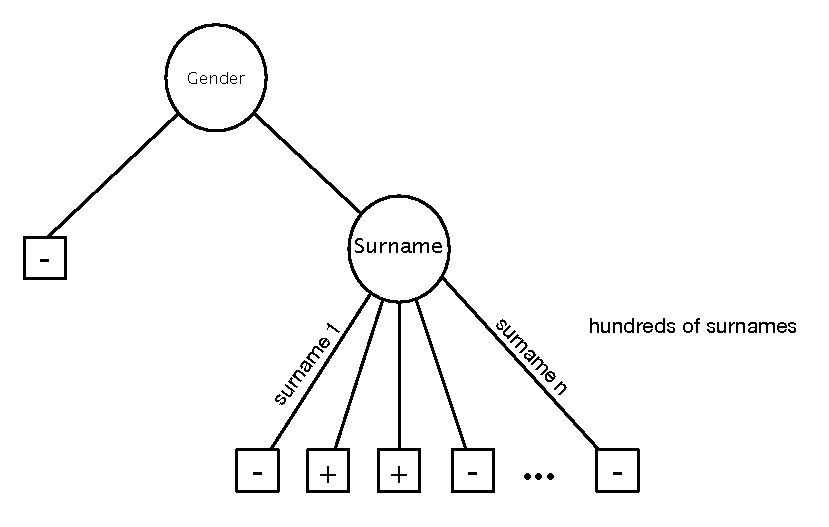
\includegraphics[width=0.9\linewidth]{fig1.pdf}
	\caption{A decision tree for the basic features}
	\label{fig:tree_base}
\end{figure}

The above example illustrates a case where, without additional knowledge, an induction algorithm will yield a very poor result. %Even if we attempt to use standard feature generation approaches, there is no additional information that combinations of these features would find.
However, if we assume access to a relational knowledge base connecting surnames to common countries of origin, we can begin to apply our knowledge-based feature generation techniques to the problem, as we can move from the domain of surnames to that of countries. 
Our algorithm does so by creating a new learning problem $T_2$. The training objects for learning problem $T_2$ are surnames; surnames of people at risk are labeled as positive. The features for these new objects are extracted from the knowledge base. In this case, we have a single feature: the country of origin.
Solving the above learning problem through an induction algorithm yields a classifier on surnames that distinguishes between surnames of patients with the disease and surnames of healthy individuals. This classifier for $T_2$ can then be used as a binary feature for the original problem $T_1$ by applying it to the feature value of surname. For example, it can be used as a feature in the node corresponding a gender of female in Figure \ref{fig:tree_base}, yielding the tree seen in Figure \ref{fig:lvl1_tree}. 

This new feature gives us a better generalization over the baseline solution, as we now abstract the long list of surnames to a short list of countries. %We can see this as nodes in the classifier for $T_2$ are derived from multiple surnames. 
This result also allows us to capture previously unseen surnames from those countries. However, this is not a sufficient solution, as we have no way of generalizing on previously unseen countries of origin. %, and some countries may not have sufficient representation to induce an accurate classifier. %talk about not concept?


\begin{figure}[h]
	\centering
	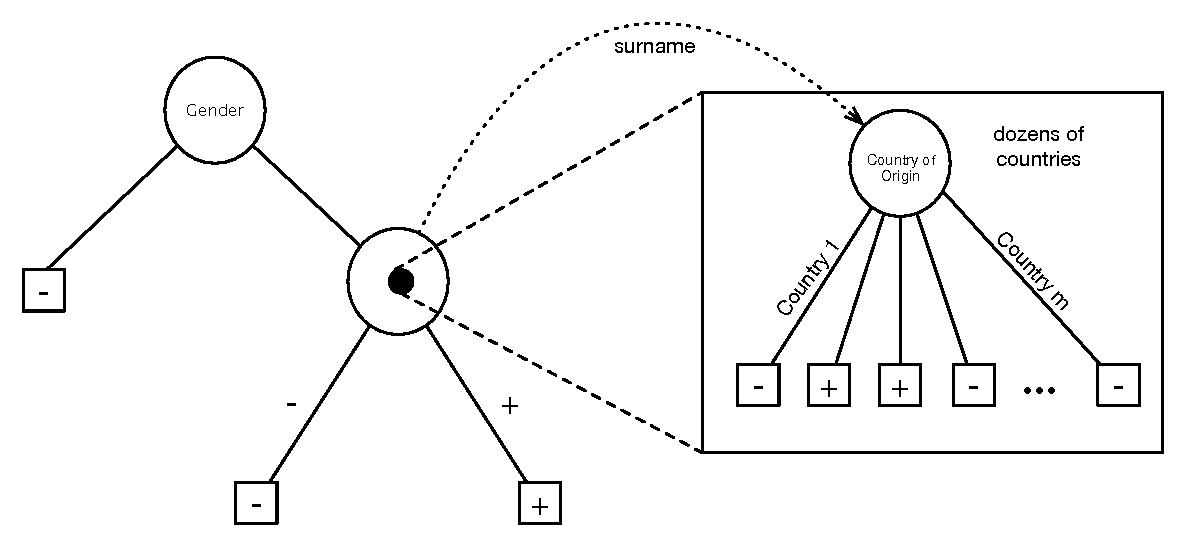
\includegraphics[width=0.9\linewidth]{fig2.pdf}
	\caption{A constructed feature used within a decision tree}
	\label{fig:lvl1_tree}
\end{figure}

If, however, we would have recursively applied our method for solving $T_2$, we could have obtained a better generalization.
When learning to classify surnames, our method creates a new learning problem, $T_3$, with countries as its objects. Countries of surnames belonging to people with high risk are labeled as positive. The knowledge base regarding countries is then used to extract features for this new training set.
Applying a standard learning algorithm to $T_3$ will yield a classifier that separates between countries of origin of people at risk and those not at risk. This classifier will do so by looking at the properties of countries, and conclude that countries with high average temperature and low precipitation, the characteristics of desert areas, are associated with people at high risk.

\begin{figure*}[th]
	\centering
	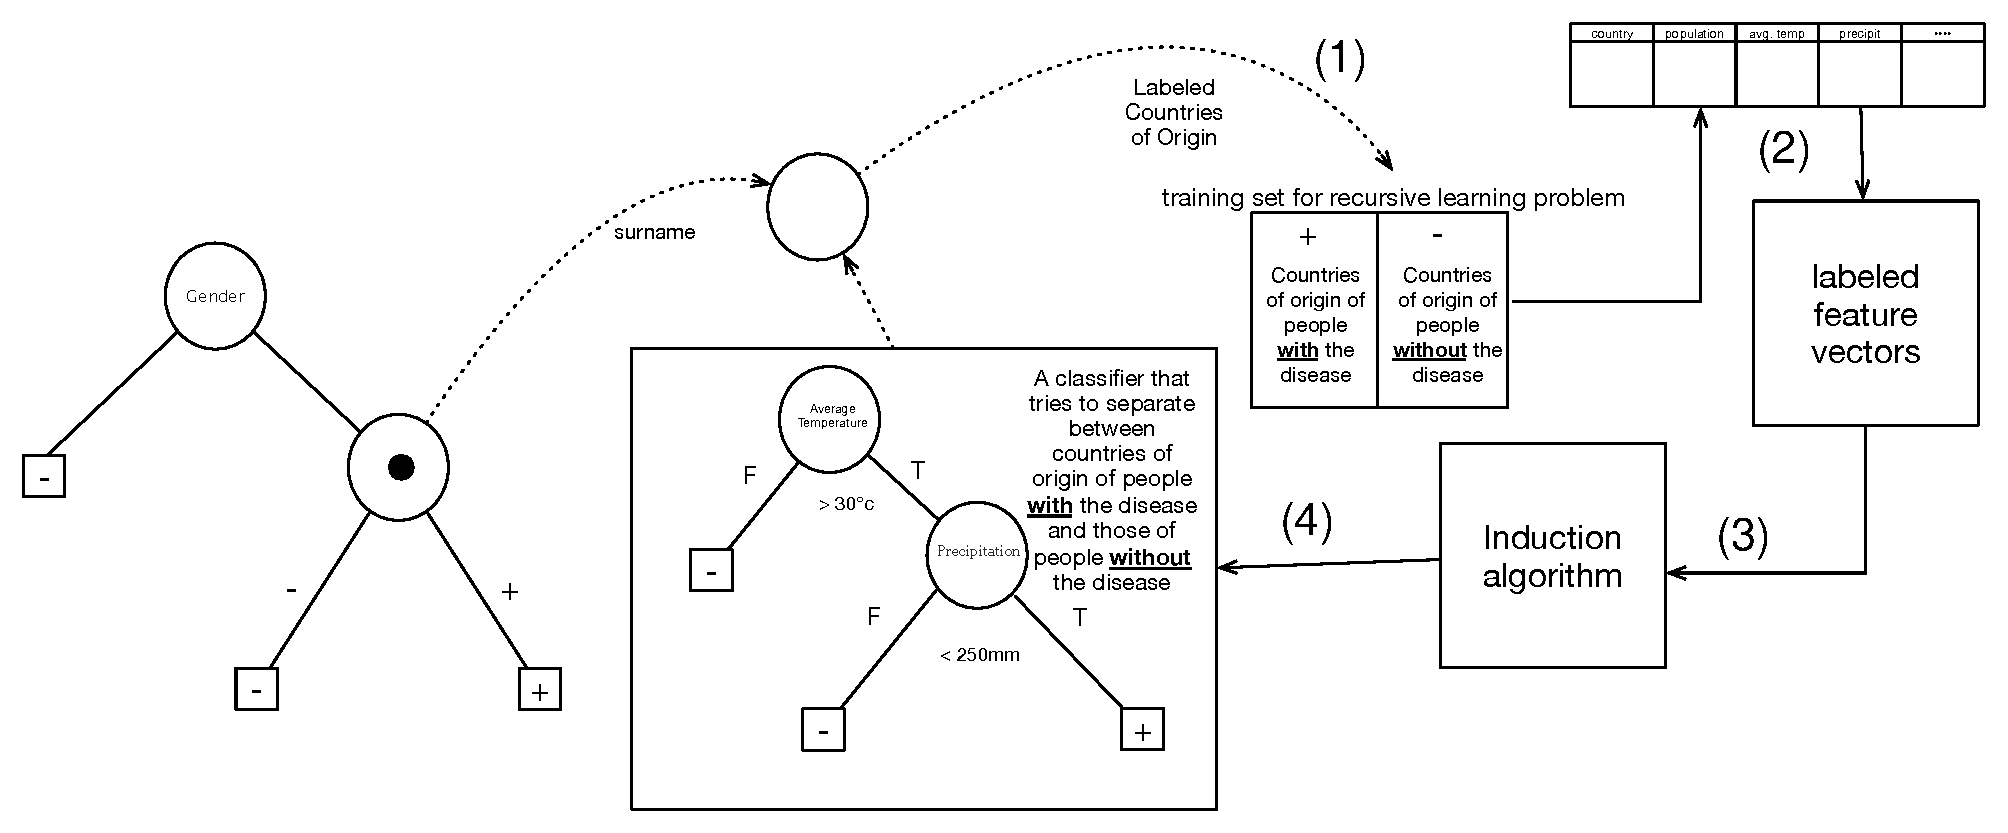
\includegraphics[width=0.9\linewidth,height=0.35\linewidth]{fig4_annotated.pdf}
	\caption{Recursive construction of a learning problem on countries of origin. $(1)$ Creating the objects for the new problem. $(2)$ Creating features using the knowledge base. $(3)$ Applying an induction algorithm. $(4)$ The resulting feature.}
	\label{fig:moving_to_lvl2}
\end{figure*}

The result of this process, depicted in Figure \ref{fig:moving_to_lvl2}, is a new feature for $T_2$, that is, a feature on surnames. This feature is then used to construct a classifier for $T_2$, which is in turn used as a feature for $T_1$, yielding a feature on patients. This new feature for patients will check whether their surname corresponds with a country of origin that has desert-like characteristics. We see that this feature allows us to correctly capture the target concept.


%\begin{figure*}[th]
%	\centering
%	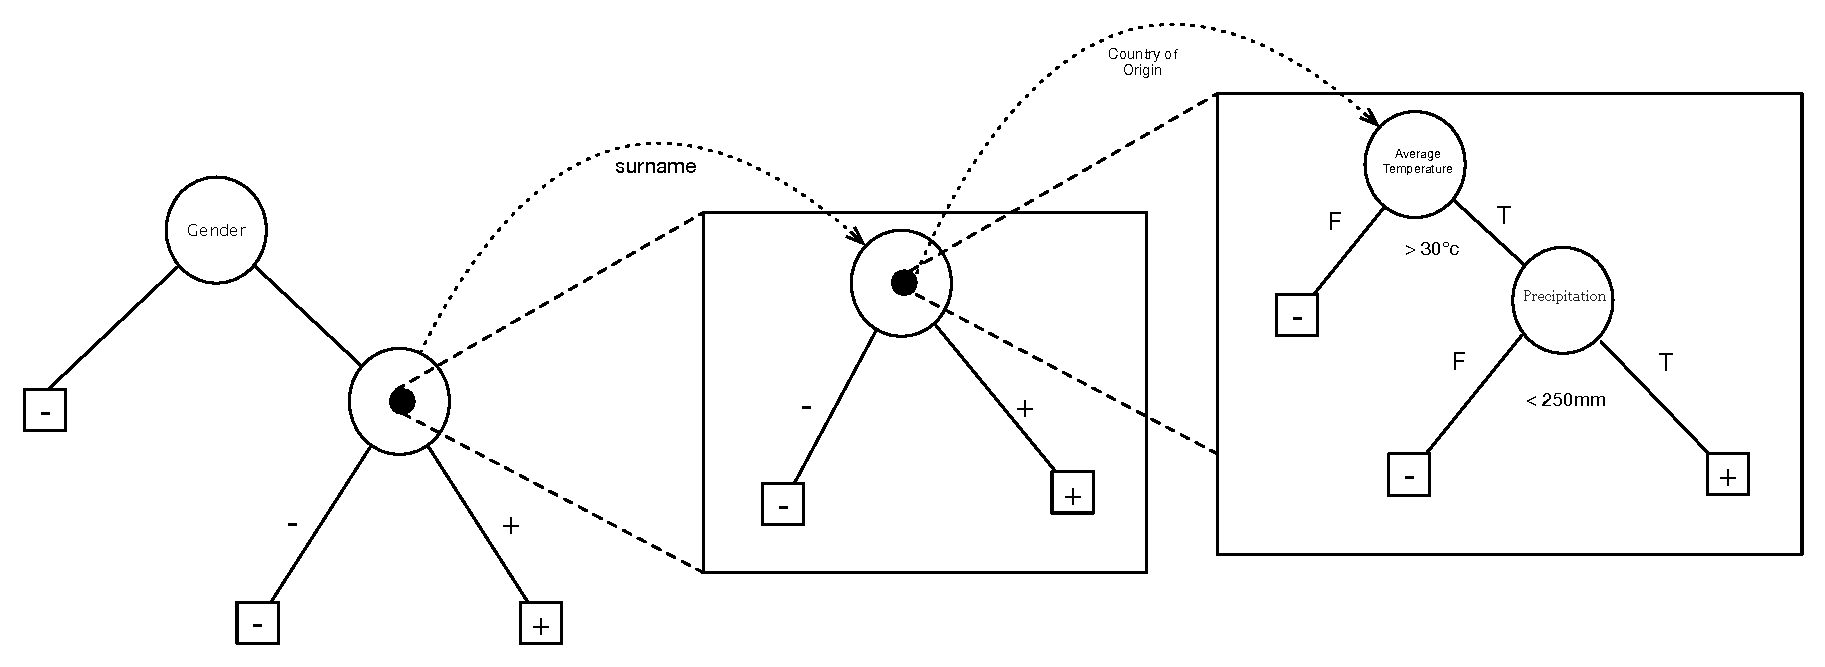
\includegraphics[width=\linewidth]{fig3.pdf}
%	\caption{A two-level constructed feature used within a decision tree}
%	\label{fig:lvl2_tree}
%\end{figure*}

%%%%%%%%%%%%%%%%%%%%%%%%%%%%%%%%%%%%%%%%%%%%%%%%%%%%%%%%%%
\section{Generating features through recursive induction} \label{formal}
%%%%%%%%%%%%%%%%%%%%%%%%%%%%%%%%%%%%%%%%%%%%%%%%%%%%%%%%%%

In the following sections, we formally define the feature generation problem, present a solution  in the form of a simple algorithm that generates features by using
relational expansions, and then proceed to describe our main recursive feature generation algorithm.

\subsection{Problem definition}

We begin our discussion with a standard definition of an induction problem. 
Let $O$ be a set of objects. Let $Y=\{0,1\}$ be a set of labels\footnote{We assume binary labels for ease of discussion.}. Let $C:O\rightarrow Y$ be a target concept. Let $S=\{(o_{1},y_{1}),\ldots,(o_{m},y_{m})\}$ be a set of labeled examples such that $o_{i}\in O, y_{i}\in Y, C(o_i)=y_i$. 
Let $F=\{f_{1},\ldots,f_{n}\}$ be a \emph{feature map}, a set consisting of \emph{feature functions} $f_{i}:O\rightarrow I_{i}$ where $I_{i}$ is the image of $f_i$.  This definition implies a training set represented by feature vectors: $S_F=\{ (\langle f_1(o_i),\ldots,f_n(o_i)\rangle, y_i) | (o_i,y_i) \in S\}$. A learning algorithm $L$ takes $S_F$ as inputs, and outputs a classifier $h_{S_F}:O\rightarrow Y$.
\begin{defn}
	Let $L(S,F)=h_{S_F}$ be the classifier given as an output by $L$ given $\langle S,F\rangle$. Assuming $S\sim D$, the generalization error of a learning algorithm $L$ is the probability $Pr(h_{S_F}(x)\neq y)$, where $(x,y)\sim D$.
\end{defn}

\begin{defn}
	A \emph{feature generation algorithm} $A$ is an algorithm that, given $\langle S,F\rangle$, creates a new feature map $F'=\{f'_{1},\ldots,f'_{k}\}, f'_{i}:O\rightarrow I_i$.
\end{defn}

In order to evaluate the output of a feature generation algorithm $A$, we must define its utility. Given $\langle S,F \rangle$, $A$ generates a feature set $F'_A$.
Let $S$ be a training set representative of the true distribution of the target concept.
Given $S$ , a feature set $F$, a generated feature set $F'_A$ and a learning algorithm $L$, the utility of $A$ is $U(A(S,F))=Pr(h_{S_F}(x)\neq y)-Pr(h_{S_{F'_A}}(x)\neq y)$, where $x\in O,y=C(x)$.

Thus, in order for the utility of $A$ to be positive, the generated feature set $F'_A$ must yield a lower generalization error than the original feature map $F$.

In this work, we assume that, in addition to $S_F$, $A$ also has access to a set of binary\footnote{If our relations are not binary, we can use projection to create multiple binary relations instead.} relations ${\cal R}=\{R_{1},\ldots,R_{t}\}, R_j:D_j\times D_{j'}$ representing our knowledge base. For each individual relation $R_j$, its set of departure is marked $D_j$ and its co-domain is denoted as $D_{j'}$. 
\begin{defn}
	A \emph{knowledge-based feature-generation algorithm} $A$ is an algorithm that, given $\langle S,F,{\cal R} \rangle$, creates a new feature map $F_{{\cal R}}=\{f'_{1},\ldots,f'_{k}\}, f'_{i}:O\rightarrow I_i$.
\end{defn}

%When using a feature generation algorithm based on a set of relations ${\cal R}$, we would like to achieve a higher utility than that achieved without the use of ${\cal R}$. We assume that some feature values are also relation keys, allowing us to apply these relations to our learning problem. More formally, we assume 
% $\bigcup_{f_i} I_i \cap \bigcup_{R_j} D_j \neq \emptyset$. 

\subsection{Expansion-based feature generation} \label{shallow_section}

In this section, we present our first method for knowledge-based feature generation that ignores the labels of the original learning problem.
The algorithm extends each feature value by all of the tuples it appears in.
Let $f_i$ be an original feature. Let $R_j:D_j\times D_{j'}$ be a relation such that  $Image(f_i) \subseteq D_j$. We can generate a new feature function $f_{i,j}:O\rightarrow D_{j'}$ by composing $R_j$ onto $f_i$, yielding our new feature function  $f_{i,j}(x)=R_j\circ f_i$.

%Another case that must be discussed is the case where some values of $f_i$ cannot be expanded as above, meaning $Image(f_i) \not\subset D_j$ but $Image(f_i) \cap D_j \neq\emptyset$. We can resolve this in a manner similar to missing features in induction problem, by treating $R_j$ as a partial function from $Image(f_i)$ to $D_{j'}$. In order to complete this partial function, we first mark \emph{undefined} as $\perp$. We can turn $R_j$ into a full function with regards to $Image(f_i)$ as follows: $\tilde{R}_j(x)=\begin{cases} R_j(x) &\mbox{if } x\in D_j\\ 
%\perp & \mbox{otherwise } \end{cases}$.
%The result is a full function $\tilde{R}_j:Image(f_i)\cup D_j\rightarrow D_{j'}\cup\{\perp\}$. We also note that the same process can be applied to cases where $R_j$ has missing values\footnote{This is usually the case in human curated knowledge bases.}, meaning it is a partial function with regards to $D_j$. 

In the general case, composing $R_j$ onto $F_i$ yields a set of values, meaning $f_{i,j}(x)=\{v\in D_{j'}|(f_i(x),v)\in R_j\}$. 
%This set can be used as a set-based feature, but since the number of possible sets is exponentially larger than the number of values, it is usually better to utilize an aggregation function on the set of values instead. 
In our work, we preferred to work on singular values rather than set-based features. To do so, we use aggregation functions.
%An aggregation function is a function that given a multi-set as input, outputs a single value. There are many types of aggregators, such as numerical aggregators (i.e. sum), categorical aggregators (i.e. most common member) and binary aggregation functions (i.e. exists).
For the experiments described in this paper, we use  
two aggregation function types: Majority and Any, but in general any other reasonable aggregation function can be used instead.
The Majority aggregator, for example, is defined as follows.  For each value $v\in D_{j'}$, we generate a binary feature function with value 1 only if $v$ is the majority value: 
$Majority^v(X)=1 \iff majority(X)=v$.
The pseudo-code of this algorithm (called   
\emph{Expander-FG}) is listed in Algorithm \ref{code-compete}.

%Now that we have considered the possible behaviours of a given relation $R_j$, we can proceed to define the \emph{Expander-FG} feature generation algorithm. Given a feature $f_i$, \emph{Expander-FG} will go over the relations within the knowledge base and attempt to create features $f_{i,j}:O\rightarrow D_{j'}\cup\{\perp\}$ through the discussed techniques. \emph{Expander-FG} then gathers all generated features and outputs them. The pseudo-code is given below.

\begin{algorithm}[H]
	\caption{\emph{Expander-FG}}
	\label{code-compete}
	\small
	$\sigma$ - An aggregation function family
	\begin{algorithmic}
		\Function{GenerateFeatures}{$S$,$F$, ${\cal R}$}
		\State $generated=\emptyset$
		\For {$f_i \in F$}
		\For {$R_j \in {\cal R}$ such that $Image(f_i)\subseteq D_{j}$ }
		\If {$R_j$ is a function}
		%\If {$Image(f_i)\subseteq D_{j}$}
		%\State add $\{f_{i,j}=R_j\circ f_i\}$ to $generated$
		\State add $\{f_{i,j}=R_j\circ f_i\}$ to $generated$
		\Else \Comment $R_j$ is a relation $R_j:D_j\times D_{j'}$
		\State add $F^\sigma_{i,j}=\{\sigma^v(f_{i,j})|v\in D_{j'}\}$ to $generated$
		\EndIf
		\EndFor
		\EndFor
		\State \Return $generated$ 
		\EndFunction
		
	\end{algorithmic}
\end{algorithm}

\subsection{Recursive feature generation algorithm}
\label{algorithm_section}
One way to extend the \emph{Expander-FG} algorithm described in the previous section is to apply it repeatedly to its own output.
Extending the algorithm in this fashion, however, would yield an exponential increase in the number of generated features.
%The approach shown in \emph{Expander-FG} has one major issue, which is that the algorithm only uses the relations for a single hop, from feature values to the relation domain.
%\begin{itemize}
%	\item The size of the generated feature set is much larger than the original f%eature set (especially when aggregation is used).
%	\item The algorithm only uses the relations for a single hop, from feature values to the relation domain.
%\end{itemize}
%We could potentially resolve this issue by applying \emph{Expander-FG} to the generated features, giving us additional hops and thus more complex features. The downside of this expansion is that it causes an exponential increase in the number of generated features.
To that end, we propose an alternative knowledge-based feature generation algorithm. Given an input $\langle S,F,{\cal R} \rangle$, for each feature $f_i\in F, f_i:O\rightarrow I_i$, our algorithm creates a recursive learning problem whose objects are the values of $f_i$, where values associated with positive examples in $S$ are labeled positive. %, and those associated with negative examples labeled negative. 
Features for this generated problem are created using the relations in ${\cal R}$. Once this new learning problem $\langle S'_i,F_{\cal R}\rangle$ is defined, an learning algorithm is used to induce a classifier $h_i:I_i\rightarrow Y$. Finally, our algorithm outputs a single generated feature for $f_i$, $f'_i(x)=h_i\circ f_i=h_i(f_i(x)), f'_i:O\rightarrow Y$.
Note that during the induction process of the newly created learning problem, we can apply a feature generation algorithm on $\langle S'_i,F_{\cal R},{\cal R} \rangle$. In particular, we can apply the above method recursively to create additional features. We call this algorithm \emph{FEAGURE} (FEAture Generation Using REcursive induction).

%\subsubsection{Creating Learning Problems using Relations}  

Given a feature $f_{i}$, we create a recursive learning problem $\langle S'_i,F_{\cal R} \rangle$. %In this section, we will discuss how we do so.
Let $v_i(S) = \{v | (o,y) \in S, f_{i}(o)=v\}$ be the set of feature values for $f_i$ in the example set $S$. %In the intro example, for instance, $v_i(S)$ will be the set of all last names of patients that appeared in the training set.
We use $v_i(S)$ as our set of objects. To label each $v \in v_i(S)$, we examine at the labels in the original problem.
If there is a single example $o \in S$ such that $f_i(o)=v$, then the label of $v$ will be the label of $o$. Otherwise, we take the majority label  $label(v)=majority(\{y|(o,y)\in S, f_i(o)=v\})$.

%We now formulate a new learning problem with the constructed training set
%$S'_i = \{ (v, label(v)) | v \in v_i(S) \}$.
To define our learning problem, we must specify a feature map over $v_i(S)$. Similarly to \emph{Expander-FG}, we use the relations in ${\cal R}$ on the elements in the new training set $S'_i = \{ (v, label(v)) | v \in v_i(S) \}$.
For each $R_j\in {\cal R}$, if it is relevant to the problem domain, meaning that $v_i(S)\subseteq D_j$, we utilize it as a feature by applying it to $v$. If $R_j(v)$ is a set, we use aggregators, as described in the previous section. 
The result of this process is a generated feature map for $S'_i$, denoted as $F_{\cal R}$. 

We now have a new induction problem $\langle S'_i,F_{\cal R} \rangle$.
We can further extend $F_{\cal R}$ by recursively using \emph{FEAGURE}, yielding a new feature map $F'_{\cal R}$. The depth of recursion is controlled by a parameter $d$, that will usually be set according to available learning resources.
We proceed to use a learning algorithm\footnote{For our experiments, we used a decision tree learner, but any induction algorithm can be used.} on $\langle S'_i,F'_{\cal R} \rangle$ in order to train a classifier, giving us $h_i:I_i\rightarrow Y$. We can then use $h_i$ on objects in $S$ as discussed above, giving us a new feature $f'_{i}(x)=h_{i}(f_{i}(x)), f'_{i}:O\rightarrow Y$. 

%TODO
The full algorithm is listed in Algorithm \ref{code-creating-prob}.
While the \emph{FEAGURE} algorithm can be used as described above, we found it more useful to use it in the context of a divide \& conquer approach, in a manner similar to the induction of decision trees.
In this approach, the set of examples is given as an input to a decision tree induction algorithm. The \emph{FEAGURE} algorithm is applied at each node. 
This allows us to generate features that are locally useful for a subset of examples.
At the end of the process the tree is discarded and the generated features are gathered as the final output.

\begin{algorithm}[H]
	\caption{FEAGURE algorithm}
	\label{code-creating-prob}
	\small
	%insert param stuff
	\begin{algorithmic}
		\Function{GenerateFeatures}{$F$, $S$, ${\cal R}$, $d$}
		\For {$f_i\in F$}
		\State $S'_i,F_{\cal R}$= \Call{CreateNewProblem}{$f_i$,$S$,${\cal R}$,$d$} %\Comment{We can apply our algorithm recursively here}
		\State $h_i$= \Call{InductionAlgorithm}{$S'_i,F_{\cal R}$} 
		%\If {\Call{Compare}{$h_i,F$}} \Comment Compare $h_i$ to $F$
		\State add $f'_i(x)=h_i\circ f_i$ to generated features
		%\EndIf
		\EndFor
		\State \Return generated features
		\EndFunction

		\Function{CreateNewProblem}{$f_{i}$, $S$, ${\cal R}$, $d$}
		\State $v_i(S) = \{v | (o,y) \in S, f_{i}(o)=v\}$
		\State Let $s(v)=\{o | (o,y)\in S, f_{i}(o)=v\}$
		\State 	$S'_i = \{ (v, \mbox{majority-label}(s(v))) | v \in v_i(S)\}$
		
		
		\State $F_{\cal R}=\{R_j(v)| R_j\in{\cal R}, v_i(S)\subseteq D_j\}$
		\If {$d>0$}
		 \State $F_{\cal R}=F_{\cal R}\cup$\Call{GenerateFeatures}{$F_{\cal R}, S'_i,  {\cal R}$, $d-1$}
		\EndIf
		\State \Return $S'_i, F_{\cal R}$ 
		\EndFunction
		
	\end{algorithmic}
\end{algorithm}

%%%%%%%%%%%%%%%%%%%%%%%%%%%%%%%%%%%%%%%%%%%%%%%%%%%%%%%%%%
\section{Empirical evaluation}
%%%%%%%%%%%%%%%%%%%%%%%%%%%%%%%%%%%%%%%%%%%%%%%%%%%%%%%%%%
We have applied our feature generation algorithm to the domain of text classification.
%In this section, we discuss our experimental methodology, detail the algorithms, datasets and knowledge bases we utilize and display our main results.

%%%%%%%%%%%%%%%%%%%%%%%%%%%%%%%%%%%%%%%%%%%%%%%%%%%%%%%%%%
\subsection{Application of \emph{FEAGURE} to Text Classification} \label{text-feagure}
%%%%%%%%%%%%%%%%%%%%%%%%%%%%%%%%%%%%%%%%%%%%%%%%%%%%%%%%%%

%assume base features, link to milne2013open,hoffart2011robust
%We use a variation of the bag-of-words \citep{Wu:1981:CST:1013228.511759} approach as the base feature set for the problem, using a single set feature whose value is a set composed of all of the words in a given document. 

%For evaluation, we use the binary bag of words representation \citep{Wu:1981:CST:1013228.511759}. This approach is not useful for our feature generation. We therefore define a virtual feature $f'$ that is used exclusively for the sake of feature generation. This $f'(e)=v iff e in enties$ 

To use \emph{FEAGURE} for text classification, we use words as binary features and Freebase and YAGO2 as our semantic knowledge bases.
YAGO2 \cite{hoffart2013yago2} is a large general knowledge base extracted automatically from Wikipedia, WordNet and GeoNames.
YAGO2 contains over 10 million entities and 124 million relational facts, mostly dealing with individuals, countries and events.
Freebase \cite{bollacker2008freebase} has been described as ``a massive, collaboratively edited database of cross-linked data." Freebase is constructed as a combination of data harvested from databases and data contributed by users. The result is a massive knowledge base containing 1.9 billion facts. 

To apply our approach to the domain of text classification, we perform a few minor adjustments to the \emph{FEAGURE} algorithm:
\begin{enumerate}
	\item To enable linkage between the basic features and the semantic knowledge bases, we use entity linking software \cite{hoffart2011robust,milne2013open} to transform these words into semantically meaningful entities.
	\item Once we have created a new classifier $h_i$, we cannot simply compose it on $f_i$, since every example might contain multiple entities. To that end,  we apply $h_i$ on each entity and take the majority vote.
	\item Since our features are binary, we use the entities extracted from the text as the set of values $v_i(S)$. We split $v_i(S)$ into several subsets according to relation domains and apply the \emph{FEAGURE} algorithm independently to each domain. 
\end{enumerate}

\subsection{Methodology}

We evaluated our performance using a total of 101 datasets from two dataset collections:

\textbf{TechTC-100} \cite{gabrilovich2004text} is a collection of 100 different binary text classification problems of varying difficulty, extracted from the Open Dictionary project.
We used the training and testing sets defined in the original paper. 
%evaluated our approach by measuring accuracy based on the training and testing sets defined in the original paper. 
As our knowledge base for this task, we used YAGO2.% \citep{hoffart2013yago2}.
%YAGO2 (Yet Another Great Ontology) is a large general knowledge base extracted automatically from Wikipedia, WordNet and GeoNames.
%YAGO2 contains over 10 million entities and 124 million facts, mostly dealing in individuals, countries and events.
%In order to fully make use of this knowledge base, we performed some processing on it. Specifically, we omitted relations with literal data such as dates or geographic coordinates, and created inverse relations of all relations except ones that map very few values to very many \footnote{For example, the inverse of the ``has gender" relation  maps ``male" and ``female" to all to all existing people within the YAGO2 database.}.

%For entity extraction, we used AIDA \citep{hoffart2011robust}, a framework for entity detection and disambiguation. %AIDA uses the Stanford NER tagger \cite{finkel2005incorporatingfull} to locate entity candidates, and attempts to link them to existing entities within the YAGO2 knowledge base.

%The TechTC-100 dataset collection served as a powerful benchmark, as it shows results for multiple problems at once, giving a broad view for many problems with varying difficulties. This aspect allowed us to better understand and analyse our approach in a variety of situations.

%We also wanted to explore the results of our approach with regards to a more domain-specific problem.
%To that end, we constructed a dataset based on OHSUMED \citep{hersh1994ohsumed}.

\textbf{OHSUMED} \cite{hersh1994ohsumed} is a large dataset of medical abstracts from the MeSH categories of the year 1991. 
%We constructed our own dataset based on the work of \cite{joachims1998text}.
First, we took the first 20,000 documents, similarly to \citeauthor{joachims1998text} \shortcite{joachims1998text}.
We limited the texts further to medical documents that contain only a title. %On each document, we used stopword elimination, a simple stemming scheme %(due to the medical nature of the texts, there was no need for complex stemming) in order to remove unnecessary noise. Once the documents have been cleaned of stopwords and stemmed,
Due to the relatively sparse size of most MeSH categories, we only used the two with the most documents, C1 and C20. %``Bacterial Infections and Mycoses" and ``Immunologic Diseases"\footnote{C1 and C20, respectively}, yielding a binary learning problem.
The result is a dataset of 850 documents of each category, for a total of 1700 documents.
We used ten-fold cross-validation to evaluate this dataset.
Since the YAGO2 knowledge base does not contain many medical relations, we used Freebase instead. We used the same data dump used by \citeauthor{bast2014easy} \shortcite{bast2014easy}. 

In our experiments, we generated features using the \emph{FEAGURE} algorithm. We then proceeded to use these new features alongside three learning algorithms: SVM \cite{cortes1995support}, K-NN \cite{fix1951discriminatory} and CART \cite{breiman1984classification}.

We compared the performance of a learning algorithm with the generated features to the baseline of the same induction algorithm without the constructed features.
In addition, since we could not obtain the code of competitive approaches for relation-based feature generation (such as FeGeLOD, SGLR), we instead compared our algorithm to \emph{Expander-FG}, which we believe to be indicative of the performance of these unsupervised approaches.

%\subsubsection{Experiment Parameters}

%We tested the following parameters: 
%\begin{enumerate}
%	\item Recursion level: We ran our feature generation algorithm for both a depth of one, creating a recursive learning problem for the original problem, and a depth of two, creating recursive learning problems within generated problems. This parameter allowed us to test the effect of both first and second order application of our feature generation approach.

%\item \emph{FEAGURE} internal induction algorithm: In section \ref{algorithm_section}, we define \emph{FEAGURE} without specifying the internal induction algorithm used to generate features within the new learning problem. We ran most of our experiments using a decision tree induction algorithm for that purpose, flattening the result to yield additional features. We also experimented with the use of other induction algorithms, namely SVM and K-NN.

%\end{enumerate}


%%%%%%%%%%%%%%%%%%%%%%%%%%%%%%%%%%%
\subsection{Results}
%%%%%%%%%%%%%%%%%%%%%%%%%%%%%%%%%%%

Table \ref{table:acc} shows average accuracies across all 10 folds for OHSUMED, as well as the average accuracies for all 100 datasets in techTC-100. When the advantage of our method over the baseline was found to be significant using a pairwise t-test (with $p<0.05$), we marked the $p$-value. Best results are marked in bold.
For the TechTC-100 dataset, \emph{FEAGURE} shows a significant improvement over the baseline approach. %, even though the number of generated features is much lower than the one achieved by the \emph{Expander-FG} algorithm, as seen in table \ref{table:features}.
Of particular note are the results for KNN and SVM, where the two-level activation of \emph{FEAGURE} (d=2) shows statistically significant improvement over \emph{Expander-FG} as well as the baseline accuracy ($p < 0.05$). 
One notable exception to our good results is the poor performance of K-NN for the OHSUMED dataset. This is likely due to the sensitivity of K-NN to the increase in dimension. 
For SVM as the external classifier, the \emph{FEAGURE} algorithm showed an improvement in accuracy for 87 of 100 datasets for $d=1$, and 91 datasets for $d=2$.
Using a Friedman test \cite{friedman1937use}, we see a significant improvement ($p<0.001$) over the baseline.
%The results for the OHSUMED datasets show that for K-NN, both feature generation methods perform poorly. %For SVM, we see a significant improvement over the baseline approach. For CART, we also see a general trend of improvement, with results for a two level application of \emph{FEAGURE} showing significant improvement over the baseline.

%Analysis of the results for the OHSUMED datasets show that for K-NN, the \emph{expander-FG} algorithm performs more poorly than the baseline approach, meaning the features generated by \emph{Expander-FG} were harmful to the induction algorithm. For \emph{FEAGURE}, we also see a degrade in accuracy, due to the masking effect inherent to K-NN classifiers, meaning that impact of a single distinguishing feature may be masked by other features, and addition of features tends to degrade performance. For SVM, we see a significant improvement over the baseline approach, with a single level application achieving an average of $2.5\%$ increase in accuracy, and a two-level application giving a total average of $2.75\%$ improvement. For CART, we also see a general trend of improvement, with results for a two level application of \emph{FEAGURE} showing significant improvement over the baseline.

\begin{table*}[th!]
	\centering
	\caption{Average accuracy over all datasets. The columns specify feature generation approach, with baseline being no feature generation. The rows specify the induction algorithm used on the generated features for evaluation.
		Results marked with * are significant with $p<0.001$.}
	\label{table:acc}
	\begin{tabular}{|l | l || l | l | l| l|}
		\hline
		Dataset & Classifier & Baseline   & Expander-FG & FEAGURE(d=1)   & FEAGURE(d=2)    \\ \hline
		\multirow{3}{*}{OHSUMED} & KNN  & \textbf{0.777} & 0.756 & 0.769   & 0.75 \\ \cline{2-6}
		& SVM  & 0.797 & 0.804   & 0.816 ($p<0.05$)    & \textbf{0.819 ($p<0.05$)} \\ \cline{2-6}
		
		& CART  & 0.806 & 0.814   & 0.809    & \textbf{0.829 ($p<0.05$)} \\
		
		\specialrule{.15em}{.05em}{.01em} % \hline
		
		\multirow{3}{*}{TechTC-100} & KNN & 0.531 & 0.702* & 0.772* & \textbf{0.775*}  \\ \cline{2-6}
		& SVM  & 0.739 & 0.782*    & 0.796*    & \textbf{0.807*} \\ \cline{2-6}
		
		& CART  & 0.81 & 0.815   & 0.814   & \textbf{0.825 ($p<0.05$)}  \\
		
		\specialrule{.15em}{.05em}{.01em}
		
		\multirow{3}{*}{TechTC-25MAA} & KNN & 0.524 & 0.723* & \textbf{0.803*} & 0.795*  \\ \cline{2-6}
		
		& SVM  & 0.751 & 0.815*   & 0.817*   & \textbf{0.829*} \\ \cline{2-6}
		
		& CART  & 0.82 & 0.839   & 0.837   & \textbf{0.849 ($p<0.05$)}  \\
		
		\specialrule{.15em}{.05em}{.01em}
		
		%	\multirow{3}{*}{TechEC-25} & KNN  & 0.539 & 0.72 ($p<0.001$) & 0.777 ($p<0.001$)  & \textbf{0.781 ($p<0.001$)} \\ \cline{2-6}
		%	& SVM  & 0.762 & 0.788  & \textbf{0.82 ($p<0.001$)}    & 0.817 ($p<0.05$) \\ \cline{2-6}
		
		%	& CART  & 0.81 & 0.833   & 0.836 ($p<0.05$)    & \textbf{0.847 ($p<0.05$)} \\
		
		%	\specialrule{.15em}{.05em}{.01em} % \hline
		
	\end{tabular}
\end{table*}

Figure \ref{fig:svm_base_lvl2} shows the accuracies for datasets in techTC-100 using a SVM classifier. The x axis represents the baseline accuracy without feature generation, and the y axis represents the accuracy using our new feature set generated using \emph{FEAGURE}. Therefore, any dataset that falls above the $y=x$ line marks an improvement in accuracy. 
The results show a strong trend of improvement, with high ($>10\%$) improvement being common.
We see that for 8 of the datasets, there is a degradation in accuracy. This can be a result of mistakes in the entity extraction and linking process.

\begin{figure}
	\centering
	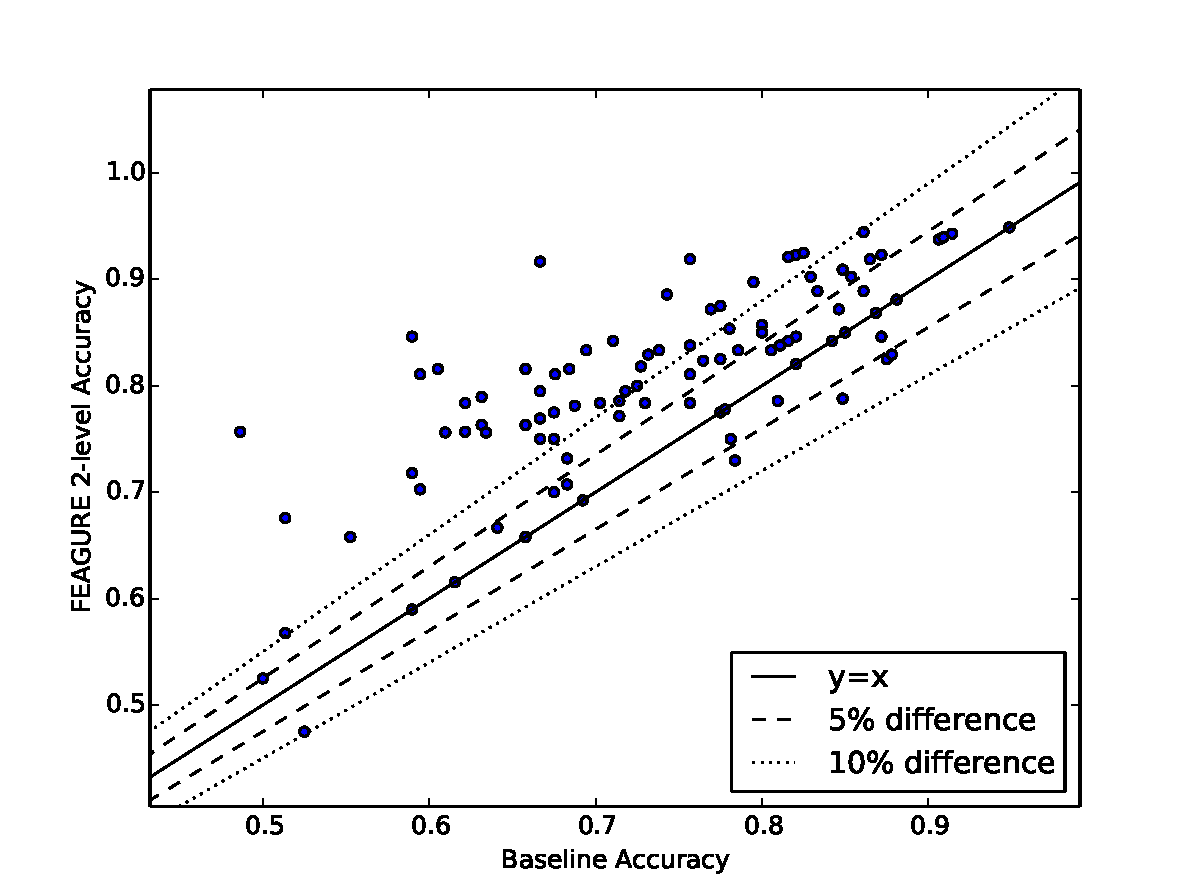
\includegraphics[width=1.0\linewidth]{svm_full_lvl2}
	\caption{Accuracy of
		baseline approach compared to two-level activation of \emph{FEAGURE} (SVM). Each point represents a dataset. The dotted lines represent a 5 and 10 percent difference in accuracy}
	\label{fig:svm_base_lvl2}
\end{figure}


In their paper on TechTC-100, \cite{gabrilovich2004text} define a metric called Maximal Achievable Accuracy (MAA). This criterion attempts to assess the difficulty of the induction problem by the maximal ten-fold accuracy over three very different induction algorithms (SVM, K-NN and CART).
%Intuitively, a dataset with low MAA can be considered harder than one with a high MAA. %, since a known induction algorithm can achieve a higher accuracy for the dataset with higher MAA. needs to be better justified(one strong == easy)
%Figure \ref{fig:25best} shows the 25 hardest datasets in TechTC-100, in terms of the MAA criterion. We call this dataset collection ``TechTC-25MAA". 
Table \ref{table:acc} also shows the accuracies for the 25 hardest datasets in TechTC-100, in terms of the MAA criterion. We call this dataset collection ``TechTC-25MAA." 
These results show a much more pronounced accuracy increase, and illustrate that we can, in general, rely on \emph{FEAGURE} to yield positive features for difficult classification problems.

As we have discussed in section \ref{algorithm_section}, \emph{FEAGURE} creates a generic learning problem as part of its execution. For our main results we learned a decision tree classifier for this new induction problem.
We also tested the effects of using K-NN and SVM classifiers instead. %, with the following parameters: For K-NN, we used $K=3$. For SVM we used $C=10$, with both Linear and a Radial Basis Function (RBF) kernels.
This choice is orthogonal to that of the learning algorithm used to evaluate the generated features.
Our experiments showed that in general, replacing the internal tree induction algorithm lowers the achievable accuracy of the resulting feature map.
The only exception to this trend is the case of an external K-NN classifier for the OHSUMED dataset. In this case, an internal RBF-SVM induction algorithm yields an average accuracy of $0.795$ (across ten folds), a significant ($p<0.05$) improvement over the baseline. 
%Table \ref{table:acc-nontree} shows the accuracies achieved by using these induction algorithms. We see that in general, with the exception of an external K-NN classifier using an internal RBF-SVM, replacing the internal tree induction algorithm is not beneficial to the accuracy of the resulting feature map.

%\begin{table*}[!th]
%	\centering
%	\caption{Average accuracy over all datasets. The columns specify the induction algorithm used in \emph{FEAGURE} (SVM with linear or RBF kernel, K-NN). The rows specify the induction algorithm used on the generated features for evaluation. Entries marked with * show a statistically significant p-value over the baseline accuracy}
%	\label{table:acc-nontree}
%	\centering
%	\begin{tabular}{|l | l || l || l | l| l|l|}
%		\hline
%		Dataset & Classifier  & Baseline & Expander-FG & Tree  & RBF SVM & 5-NN    \\ \hline
		
%		\multirow{3}{*}{OHSUMED} & KNN  & 0.777 & 0.756 & 0.769 & \textbf{0.795*}   & 0.771 \\ \cline{2-7}
%		& SVM  & 0.797 & 0.804 & \textbf{0.816*}   & 0.796    & 0.788 \\ \cline{2-7}
		
%		& CART  & 0.806 & \textbf{0.814} & 0.809   & 0.791    & 0.787 \\
		
%		\specialrule{.15em}{.05em}{.01em} % \hline
		
%		\multirow{3}{*}{TechTC-100} & KNN & 0.531 & 0.702* & \textbf{0.772*} & 0.689*   & 0.705*\\ \cline{2-7}
%		& SVM   & 0.739 & 0.782* & \textbf{0.796*}  & 0.774*   & 0.774* \\ \cline{2-7}
		
%		& CART & 0.81 & \textbf{0.815} & 0.814   & 0.81    & 0.79 \\
		
%		\specialrule{.15em}{.05em}{.01em} % \hline
		
		%\multirow{3}{*}{TechTC-25H} & KNN & 0.524 & 0.723* & \textbf{0.803*} & 0.744* & 0.7239*   & 0.724*\\ \cline{2-8}
		%& SVM   & 0.751 & 0.815* & \textbf{0.817*} & 0.794*  & 0.799*   & 0.782* \\ \cline{2-8}
		
		%& CART & 0.82 & \textbf{0.839} & 0.837 & 0.786   & 0.799    & 0.801 \\
		
		%\specialrule{.15em}{.05em}{.01em} % \hline
		
%	\end{tabular}
%\end{table*}

\subsection{\emph{FEAGURE} Demonstration}

To demonstrate \emph{FEAGURE}, We selected one problem from TechTC-100. In this example, texts refer either to locations in and around Texas, or to locations in and around New York. The extracted entities are locations, with the ``Located in" relation as our domain (Figure \ref{fig:figure_rec3_example}). Applicable relations are used to then create a new induction problem. \emph{FEAGURE} uses the ``Located in" and ``Happened in" relations as features for this problem, as shown in Figure \ref{fig:figure_rec3_problem}. 

\begin{figure}[!h]
	\centering
	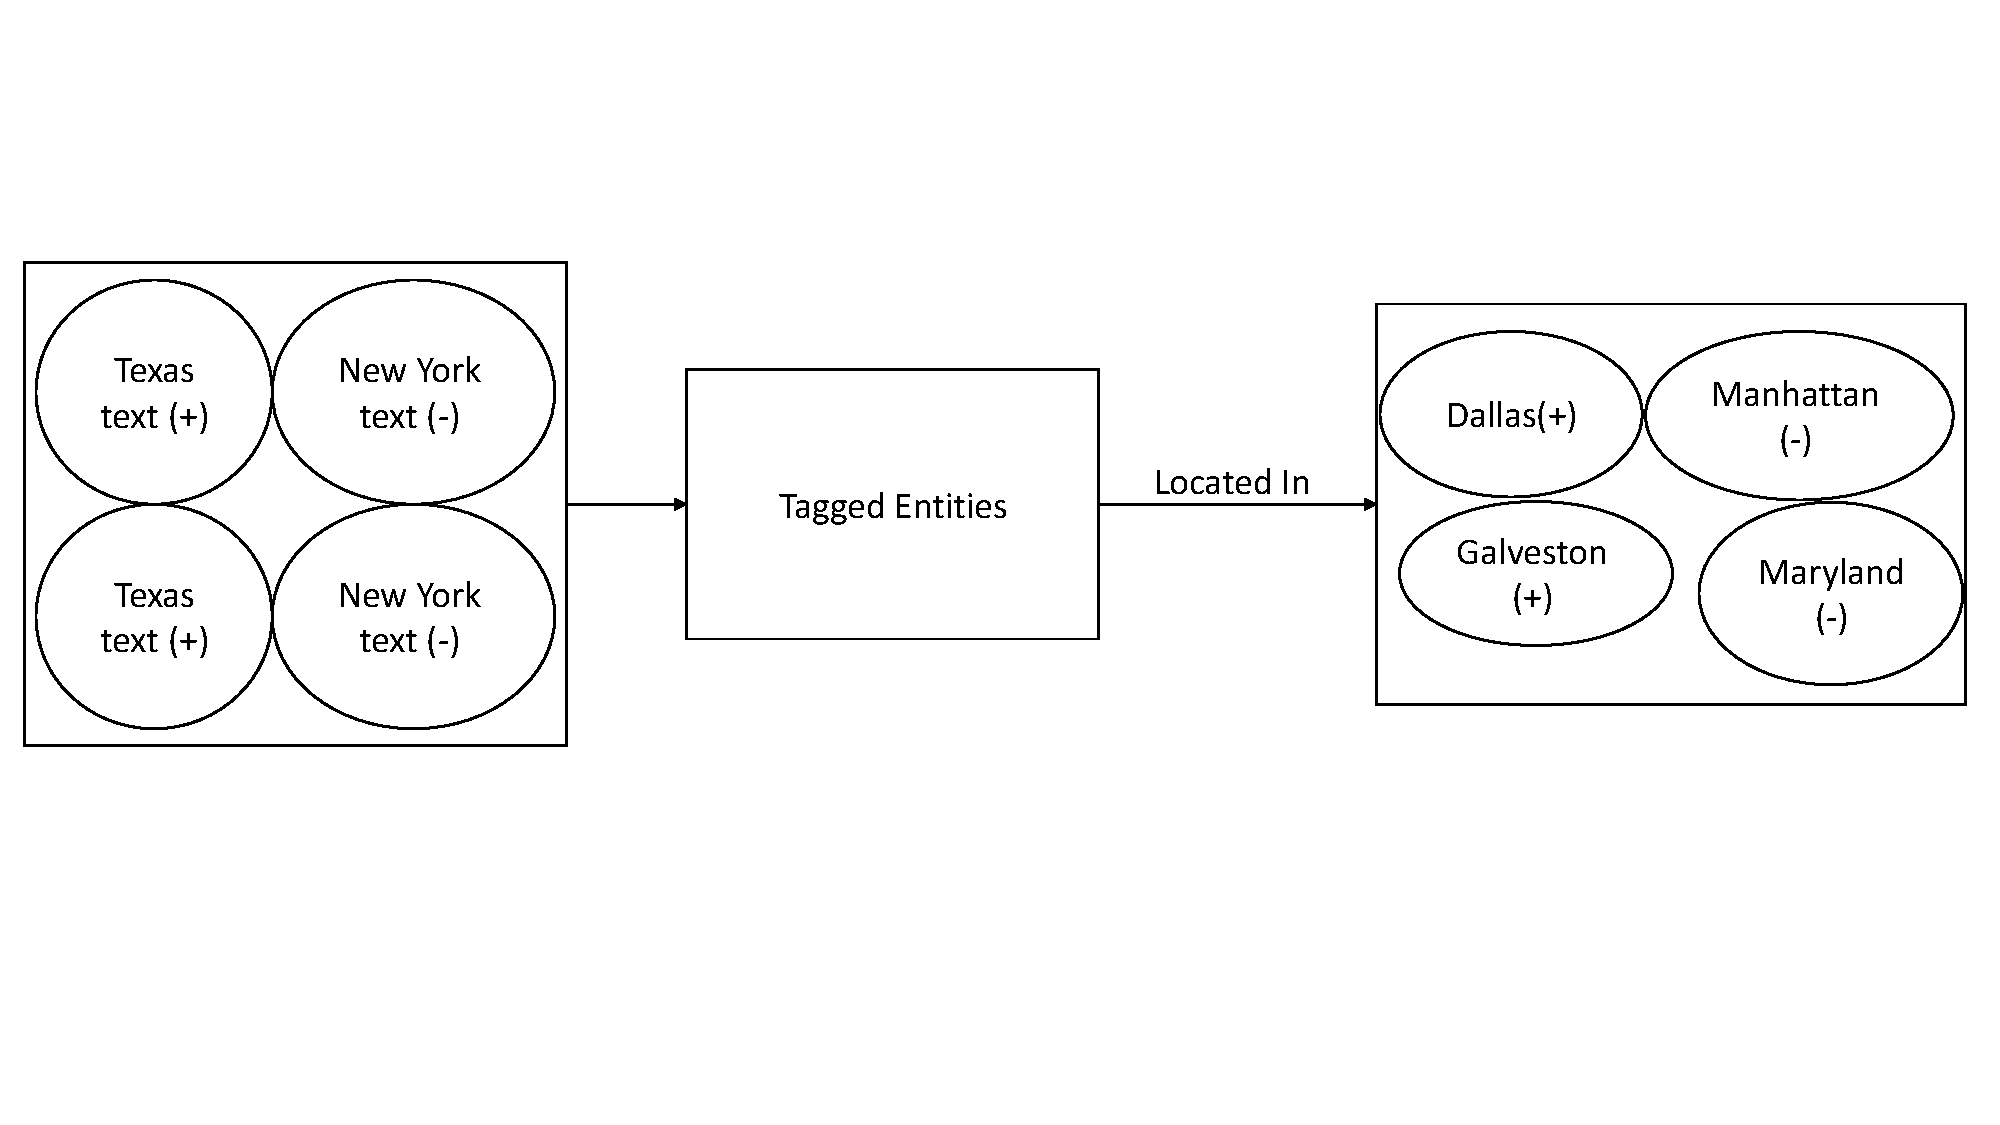
\includegraphics[width=\linewidth]{figure_rec3_example_new}
	\caption{Entities are extracted from the text, and entities in the ``Located in" relation are used as labeled objects.}
	\label{fig:figure_rec3_example}
\end{figure}

\begin{figure}[!h]
	\centering
	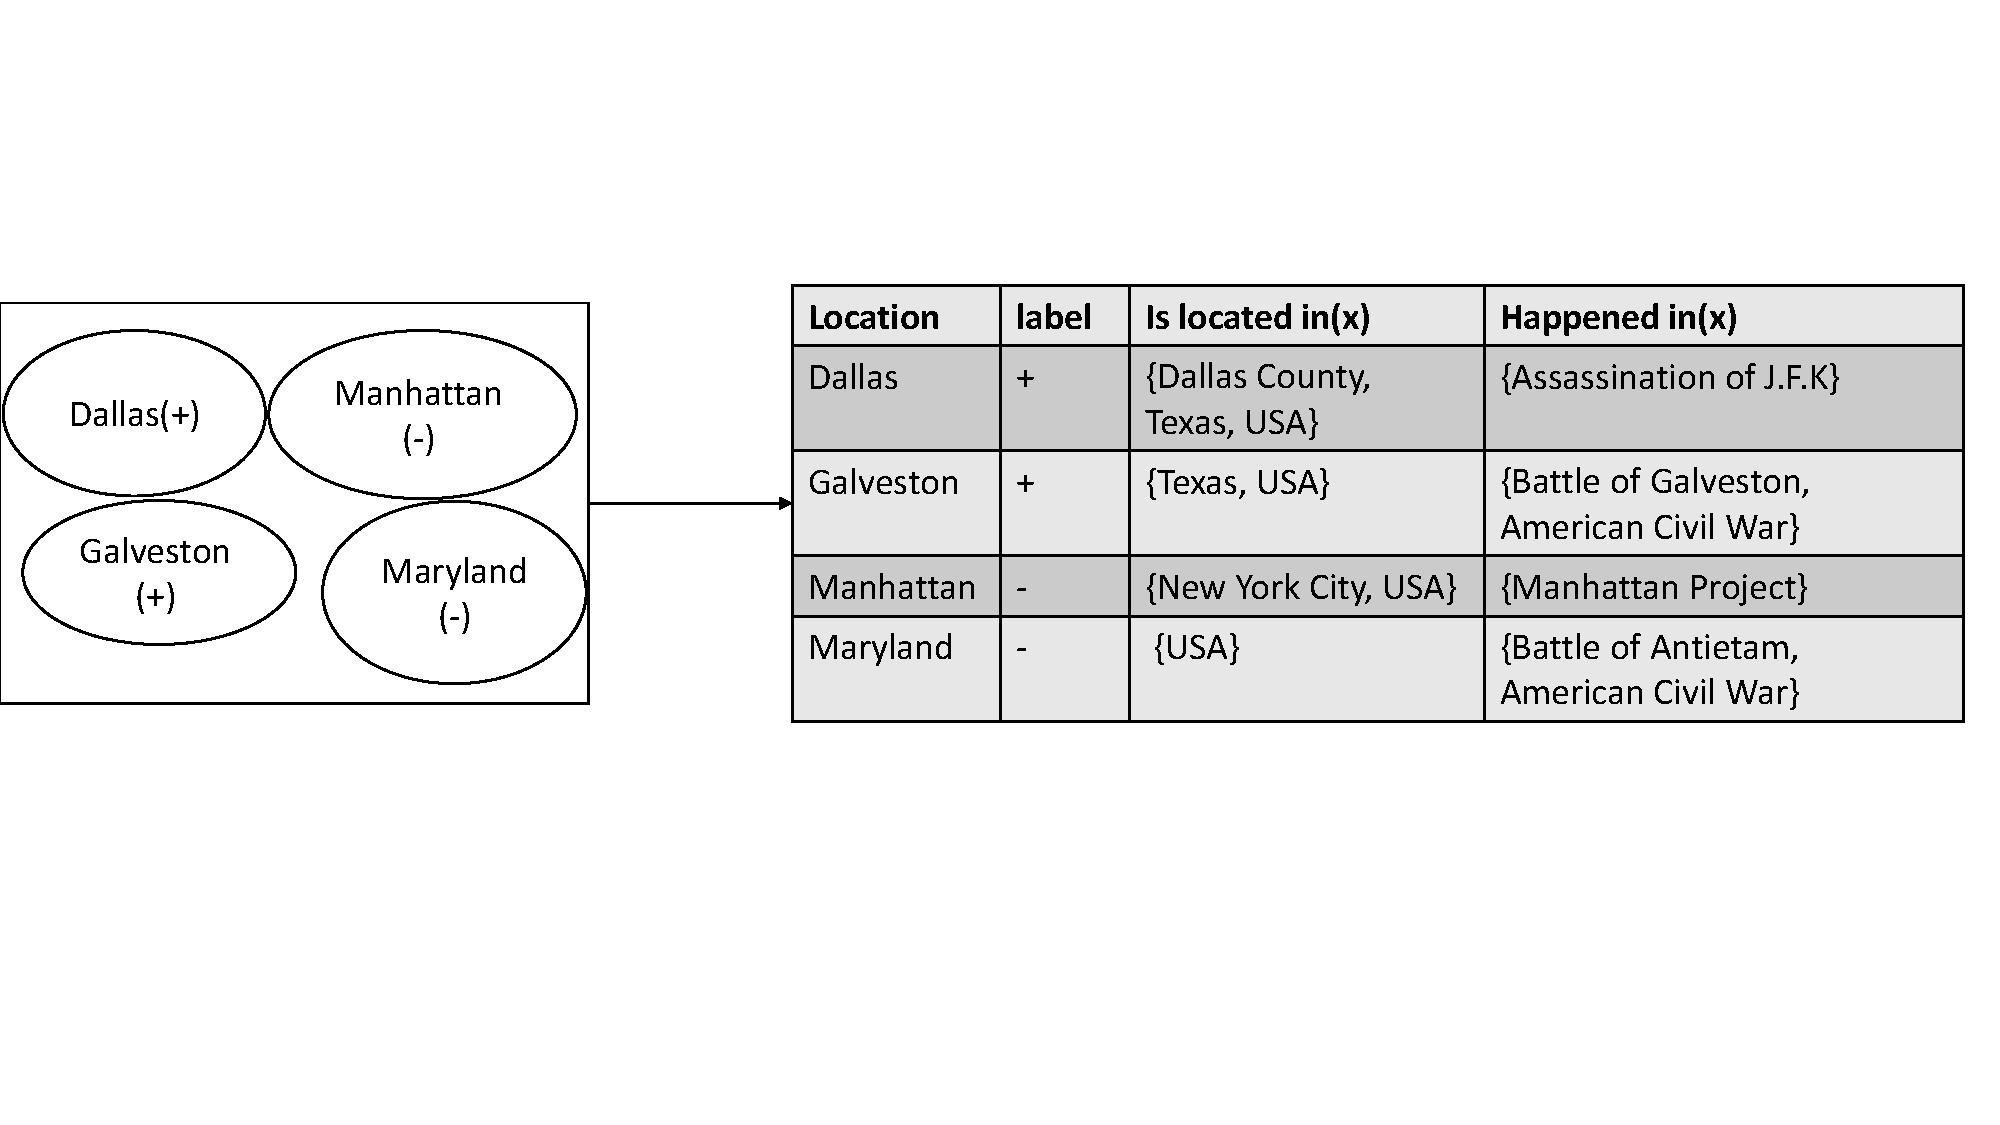
\includegraphics[width=\linewidth]{figure_rec3_problem_new}
	\caption{Construction of a recursive learning problem based on the ``Located in" relation. Applicable relations are used to create a feature set for the newly constructed example set.}
	\label{fig:figure_rec3_problem}
\end{figure}

Since we chose $d=2$ as the recursion depth parameter, the algorithm calls \emph{FEAGURE} recursively to try and generate new features for the new induction problem.
The values of the feature ``Happened in" are events. These events are used as objects for a recursive learning problem (Figure \ref{fig:figure_rec3_example_rec}).
We use the ``Type" relation as a feature, relying on hypernyms to classify events (Figure \ref{fig:figure_rec3_problem_rec}).
The resulting classifier (a decision tree induction algorithm was used) is shown in Figure \ref{fig:figure_rec3_feature}, and can be interpreted as ``is this event a battle or conflict?".

\begin{figure}[!h]
	\centering
	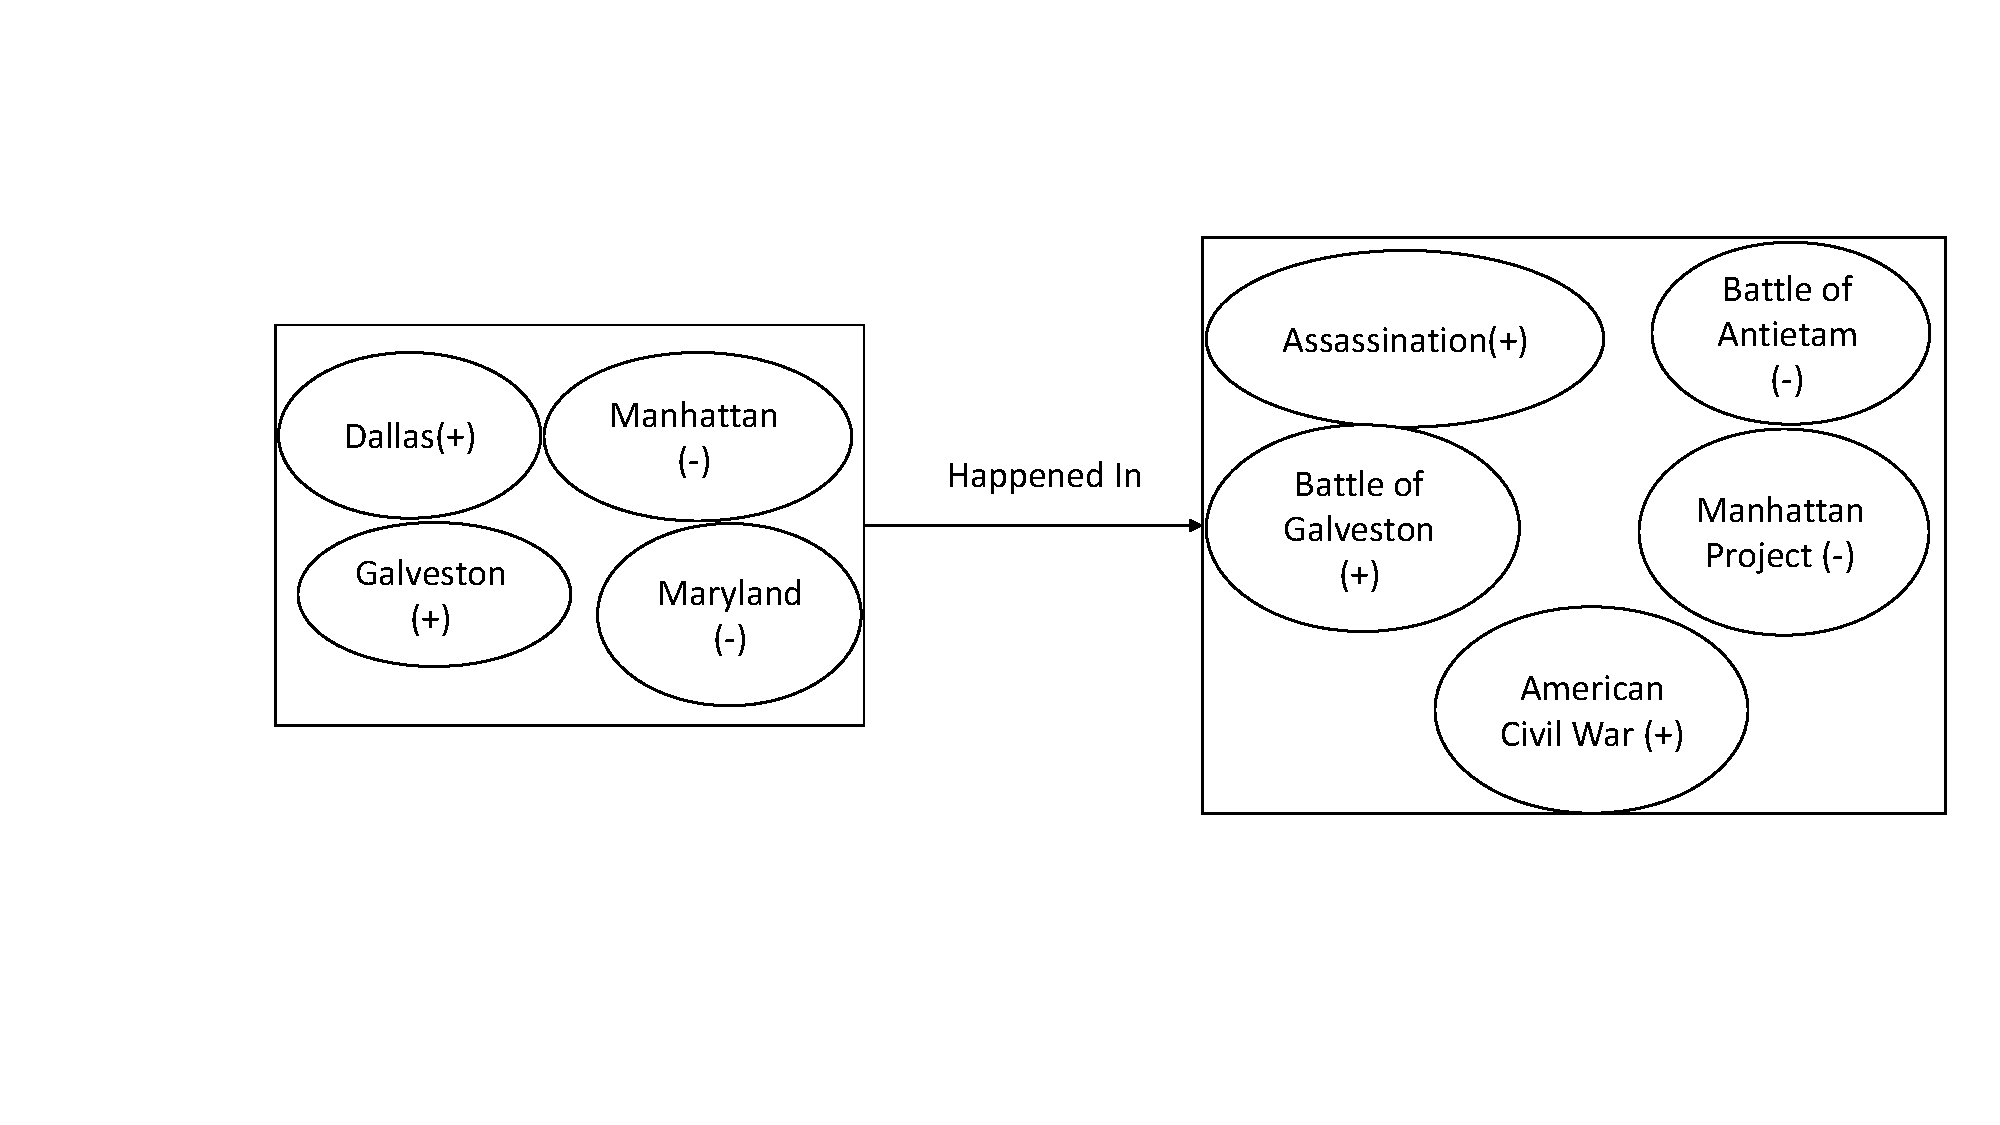
\includegraphics[width=\linewidth]{figure_rec3_example_rec_new}
	\caption{Construction of a second level recursive learning problem based on the ``Happened in" relation. Feature values are treated as objects and labeled according to the labels of the problem on locations.}
	\label{fig:figure_rec3_example_rec}
\end{figure}

\begin{figure}[!h]
	\centering
	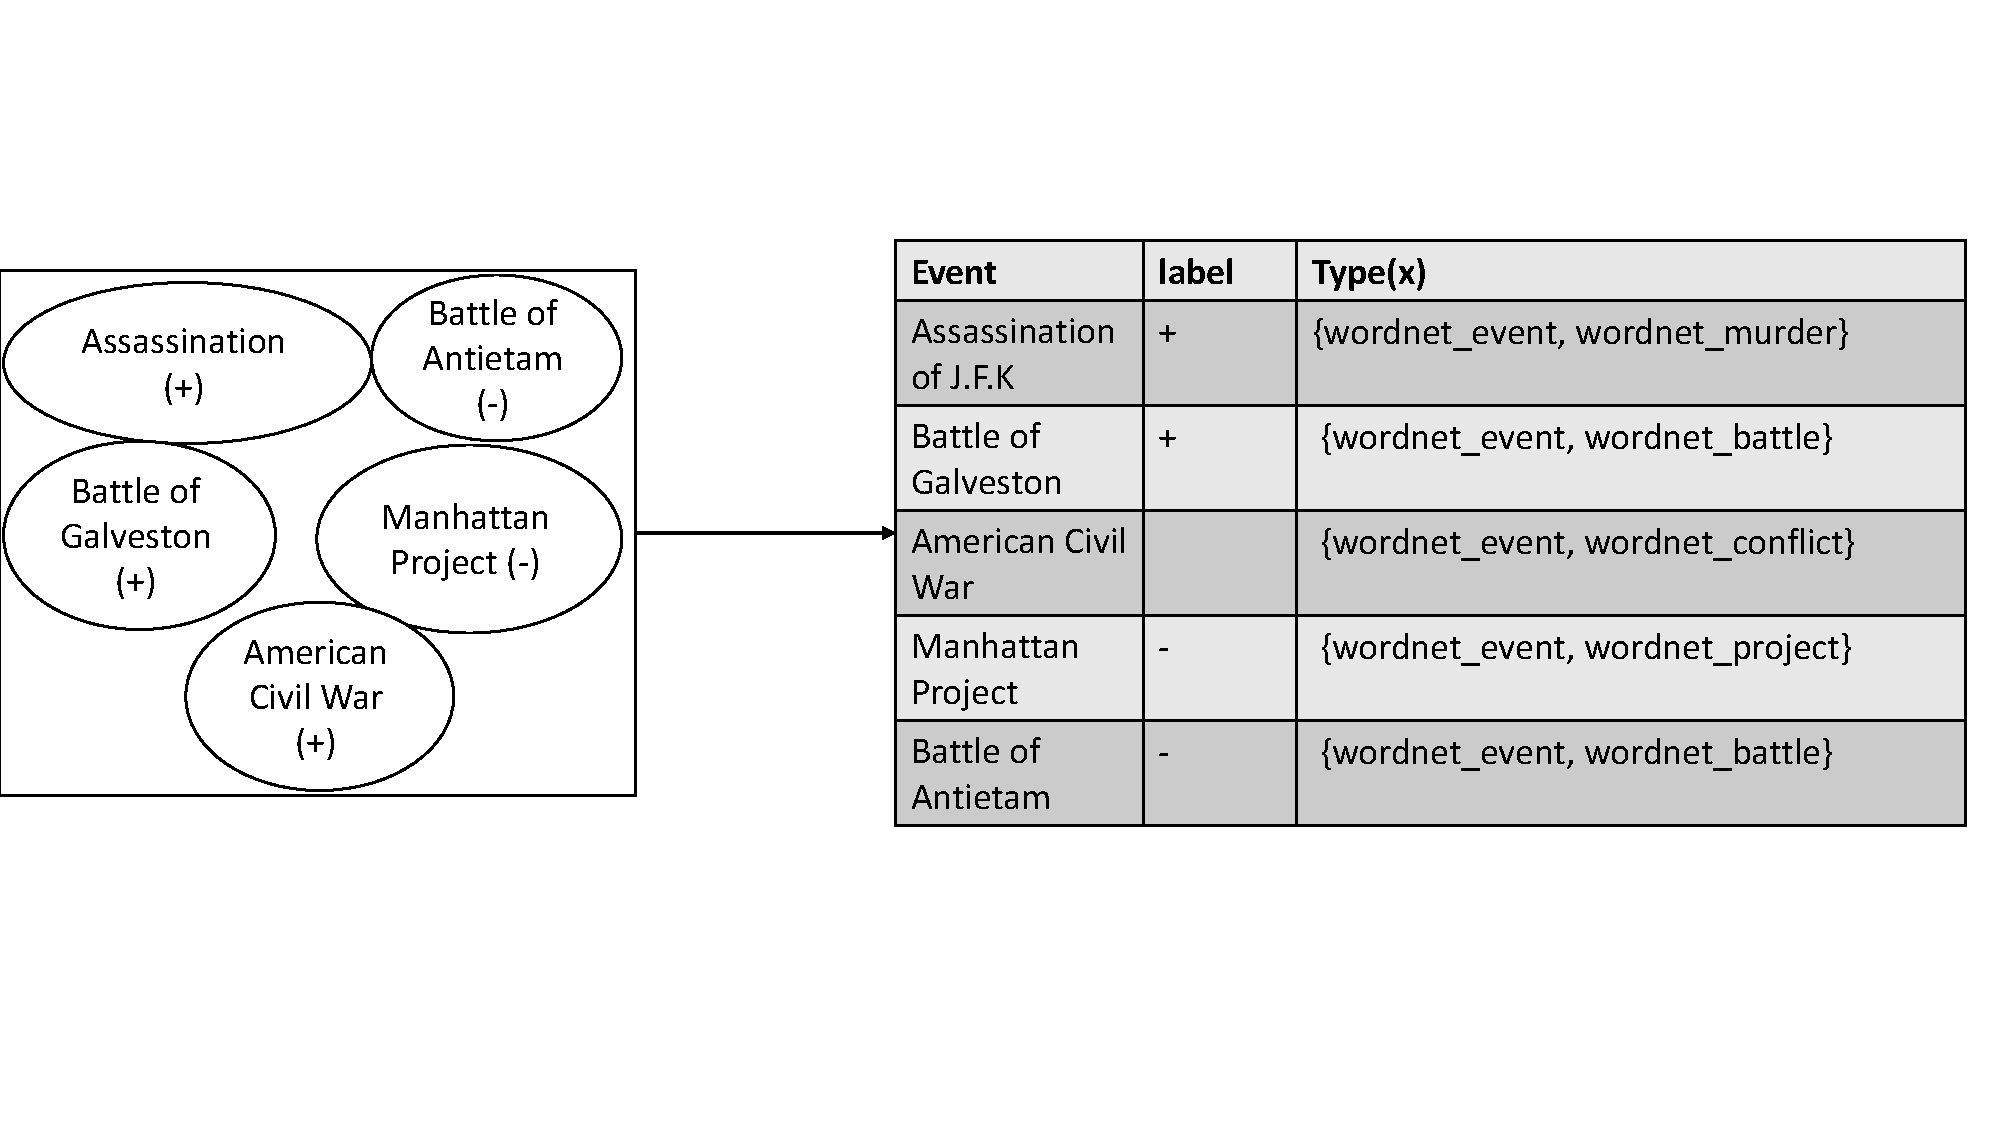
\includegraphics[width=\linewidth]{figure_rec3_problem_rec_new}
	\caption{Construction of a recursive learning problem based on the ``Happened in" relation. Once the example set has been created, applicable relations are used to create a feature set for the newly constructed induction problem.}
	\label{fig:figure_rec3_problem_rec}
\end{figure}

\begin{figure}[!h]
	\centering
	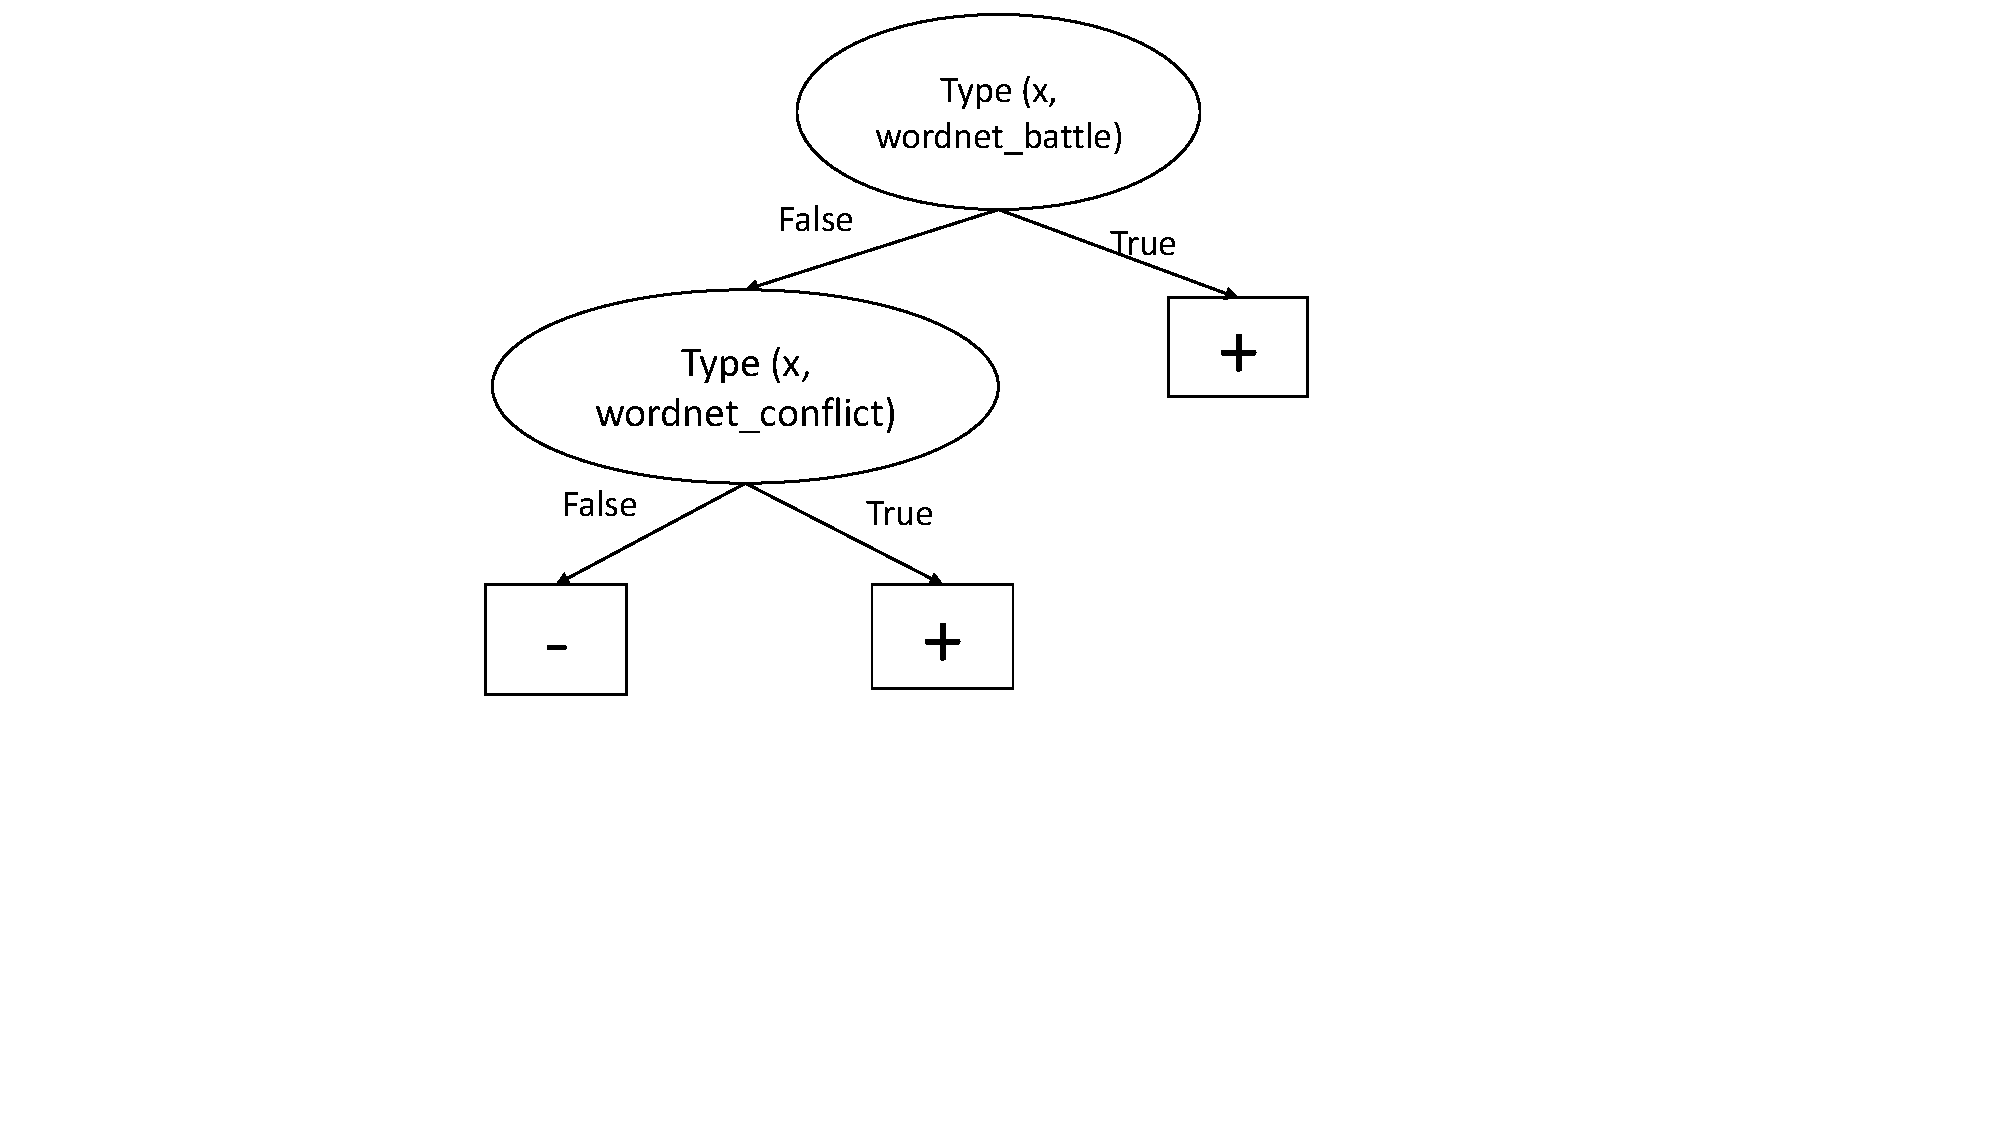
\includegraphics[width=0.7\linewidth]{figure_rec3_feature_rec_new}
	\caption{Recursive feature constructed by \emph{FEAGURE} for entities in the ``happened in" relation. This feature operates on events, and can be used in a classifier on locations.}
	\label{fig:figure_rec3_feature}
\end{figure}

Once we have generated this classifier on events, we can use it as a binary feature. \emph{FEAGURE} uses this new feature to expand the constructed induction problem on locations, shown in Figure \ref{fig:figure_rec3_problem}.
This feature is applied to a location through a majority vote over events that happened in that location. The result is a feature for locations representing the concept ``were most notable events in this location battles/conflicts?"
Finally, a decision tree learner is used on the expanded feature set to learn a classifier on locations to be used as a feature for our original learning problem. The new classifier for locations is shown in Figure \ref{fig:figure_rec3_feature_full}. It can be described as ``is this location located in Texas, or the site of battles or conflicts?".
Texts mentioning locations in and around Texas are more likely to link to locations that correspond to the output of this classifier.
We note that this feature was generated by \emph{FEAGURE}, and was later used by our external induction algorithm due to its high information gain. 

\begin{figure}[!h]
	\centering
	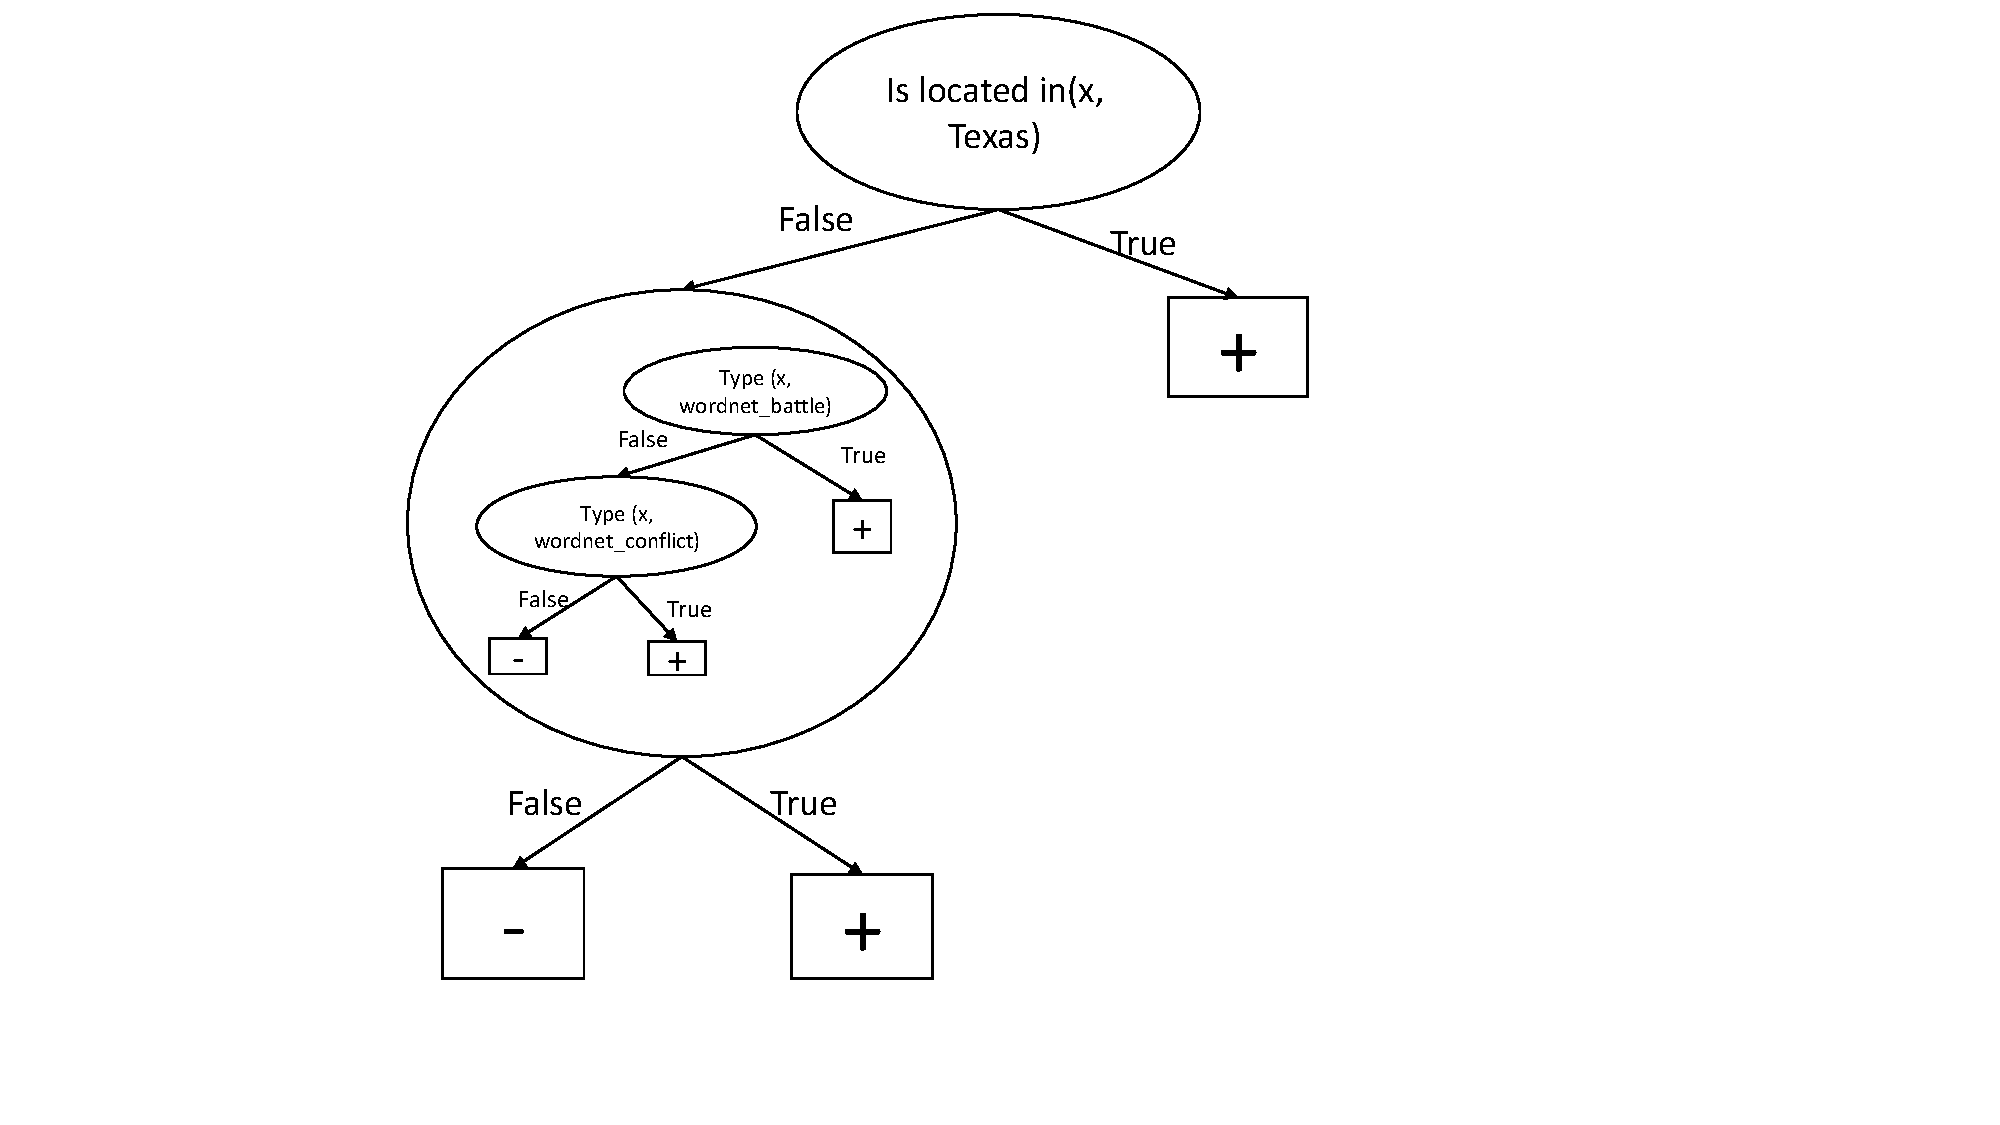
\includegraphics[width=\linewidth]{figure_rec3_feature_new}
	\caption{Final generated feature constructed by \emph{FEAGURE} for entities in the ``located in" relation. The feature in the left branch is the recursive feature constructed by applying \emph{FEAGURE} to the new learning problem.}
	\label{fig:figure_rec3_feature_full}
\end{figure}

\section{Related work}

Many feature generation methodologies have been developed to search for new features that better represent the target concepts. There are three major approaches for feature generation: tailored methods, combinational techniques and algorithms utilizing external knowledge.

Tailored approaches \cite{sutton1991learning,hirsh1994bootstrapping} are designed for specific problem domains and rely on domain-specific techniques. %for feature construction. 
%One such example is the bootstrapping algorithm \cite{hirsh1994bootstrapping}, which was designed for the domain of molecular biology. The algorithm represents features as nucleotides sequences
%whose structure is determined by existing background knowledge. The algorithm uses an initial set of feature sequences, produced by human experts, and uses a domain-specific set of operators to alter them into new sequence features. 
Such special-purpose algorithms % may be effectively tailored for a given domain, but 
have proven difficult to generalize to other domains and problems.

Combinational feature generation techniques are domain-independent methods for constructing new features by combining existing features. The LDMT algorithm \cite{utgo1991linear} performs feature construction in the course of building a decision-tree classifier. At each tree node, the algorithm constructs a hyperplane feature through linear combinations of existing features in a way likely to produce concise, relevant hyperplanes. The LFC algorithm \cite{ragavan1993complex} combines binary features through the use of logical operators such as $\land ,\lnot$.
The FICUS algorithm \cite{markovitch2002feature} allows the use of any combinational feature generation techniques, based on an a given set of constructor functions. Recent work by \citeauthor{katz2016explorekit} \shortcite{katz2016explorekit} uses a similar approach.
\emph{Deep Learning} \cite{rumelhart1986learning,lecun1998gradient} is another major class of combinational feature generation approaches. Here, the activation functions of the nodes can be viewed as feature schemes, which are instantiated during the learning process by changing the weights.

One limitation of combinational approaches is that they merely combine existing features to make the representation more suitable for the 
learning algorithm. 
%Another class of feature generation algorithms seek to inject additional knowledge into the existing learning problem.
Our \emph{FEAGURE} algorithm belongs to a third class of approaches that inject additional knowledge into the existing problem through the feature generation process.

Propositionalization approaches \cite{kramer2000bottom,cheng2011automatedfull} rely on relational data to serve as external knowledge. They use several operators to create first-order logic predicates connecting existing data and relational knowledge. 
\citeauthor{cheng2011automatedfull} \shortcite{cheng2011automatedfull} devised a generic propositionalization framework  using linked data via relation-based queries. 
FeGeLOD \cite{paulheim2012unsupervisedfull} also uses linked data to automatically enrich existing data. 
FeGeLOD uses feature values as entities and adds related knowledge to the example, thus creating additional features. 

Unsupervised approaches allow us to utilize external knowledge, but they have a major issue: Should we try to construct deep connections and relationships within the knowledge base, we would experience an exponential increase in the number of generated features.
To that end, \emph{FEAGURE} and other supervised approaches use the presence of labeled examples to better generate deeper features.

%Unlike unsupervised approaches, some methods, \emph{FEAGURE} included, seek to utilize a labelled training set in order to perform a more guided search through the space of possible features based on external knowledge. 
%Most of these techniques can trace their source to \emph{Inductive Logic Programming (ILP)} \citep{muggleton1991inductive, quinlan1990learning}, a supervised approach that induces a set of first-order logical formulae with the purpose of achieving a good separation of the given training set. 
%ILP methods do so by starting from single relation formulae and adding additional relational constraints using the knowledge base, until formulae that separate the training set into positive and negative examples are found. To that end, these approaches make use of an operator known as a refinement operator. When applied on a relational formula, a refinement creates a more specialized case of that formula. For example, given the logical formula $BornIn(X,Y)$, where $X$ is a person and $Y$ is a city, one possible refinement is the formula $BornIn(X,Y)\land CapitalOf(Y,Z)$, where $Z$ is a country. The result is a logical formula that considers a more specific case. Additionally, we can look at a refinement that restricts by a constant, turning $BornIn(X,Y)$ into, for example, $BornIn(X, \mbox{{United States}})$.This refinement process continues until a sufficient set of consistent formulas is found.
%TODO: muggleton is super important

%An algorithm suggested by \cite{terziev2011feature} shows an interesting approach to supervised feature generation. In his paper, \cite{terziev2011feature} suggests a decision tree based approach, where in each node of the tree, an expansion of features is done similarly to FeGeLOD, with a criteria based on entropy used to decide whether further expansion is required. This technique bears several similarities to the approach of \emph{Deep-FEAGURE} (Algorithm \ref{code-tree-thing}). Unlike Deep \emph{FEAGURE}, the feature expansion process is unsupervised, and the resulting feature must be a decision tree, restricting the generality of the approach.

The \emph{dynamic feature generation} approach used by the SGLR algorithm \cite{popescul200716} can be seen as the supervised equivalent of propositionalization methods. Feature generation is performed during the training phase, allowing for complex features to be considered by performing a best-first search on possible candidates.
This process allows SGLR to narrow the exponential size of the feature space to a manageable number of candidates.
While this supervised approach overcomes the exponential increase in features that unsupervised approaches suffer from, the space of generated features that it searches is significantly less expressive than that of our approach.
Through the use of recursive induction algorithm, our approach automatically locates relationships and combinations that we would not consider otherwise.

Two examples of text-based approaches for feature generation are 
Explicit Semantic Analysis (ESA) \cite{gabrilovich2009wikipediafull} that generates explicit concepts from Wikipedia, and Word2Vec \cite{mikolov2013distributed} that generates latent concepts based on a large corpus. 

%One known method of utilizing external knowledge is known as Deductive Learning \citep{mitchell1982generalization,dejong1986explanation}. This school of learning methods uses a knowledge base of logical assertions in order to locate a small set of logical conditions that capture the target concept based on examples from that concept. This approach does so using deduction, rather than induction, as its main tool, allowing us to leverage a logical knowledge base effectively.
%There are two main concerns that must be addressed for deductive learning to be effective:
%\begin{enumerate}
%	\item Extensive knowledge bases comprised of logical assertions are difficult to find and create.
%	\item This approach forfeits the progress and power gained by the use of well-known and extensively researched inductive methods.
%\end{enumerate}

%Another type of supervised, knowledge-based, feature generation approaches is \emph{Relational Learning} techniques. These techniques are designed to utilize relational databases and expand their knowledge. One such technique is that of View Learning \cite{davis2005view}. View learning generates new relational tables from the existing relational knowledge, based on labelled data.
%It does so by applying ILP on relational data to construct new, simple, relational tables, then using a Bayesian network induction algorithm, learns ways in which these relations can be combined more effectively into a single, more complex table.
%This approach bears similarity to our approach in that it can effectively utilize background knowledge to draw conclusions using the combination of labelled data and background knowledge. Unlike our approach, these views attempt to fit new knowledge to existing examples, whereas our approach re-frames the learning problem within a new context.

%Kernel-based knowledge injection techniques aim to make use of powerful machine learning algorithms such as SVM and Deep-learning techniques by decoupling the knowledge base from the induction algorithm. This is done through the use of a kernel function that acts as a similarity function between examples in the problem domain. An example of this approach can be seen in the work of \cite{losch2012graph}, which attempts to learn graph kernels within the relational domain. This creates strong kernel functions that look at the neighbourhood of an entity in search of similarities between entities. This approach bears some similarity to our own in that it can locate complex relationships, but they fundamentally differs in their approach. Kernel methods attempt to create a filter through which entity similarity can be measured. In our approach, we attempt to locate the target concept through the use of different domains. This distinction is especially relevant to classification tasks, where many possible domains can apply for each example, and similarity may be difficult to find when considering the entire example set.

\section{Conclusions}
%finishing up and summary

When humans use inductive reasoning to draw conclusions from their experience, they use a vast amount of general and specific knowledge. In this paper we introduced a novel methodology for enhancing existing learning algorithms with background knowledge represented by relational knowledge bases.
The algorithm works by generating complex features induced using the available knowledge base. It does so through the extraction of recursive learning problems based on existing features and the knowledge base, that are then given as input to induction algorithms. The output of this process is a collection of classifiers that are then turned into features for the original induction problem.

With the recent surge of well-formed relational knowledge bases,
and the increase in use of strong learning algorithms for a wide variety of tasks,
we believe our approach can take the performance of existing machine learning techniques to the next level.
%our approach can serve as a bridge between machine learning and semantic knowledge.

%% The file named.bst is a bibliography style file for BibTeX 0.99c
\clearpage
\bibliographystyle{aaai}
\bibliography{document}

\end{document}

